\documentclass[twoside,openright]{uva-bachelor-thesis}

%\usepackage[dutch]{babel} % uncomment if you write in dutch
\usepackage{graphicx}
\usepackage{url}
\usepackage{mathtools}
\usepackage{amsmath}
\usepackage{caption}
\usepackage{subcaption}
\usepackage{cite}


% Title Page
\title{The Giving Game}
\author{Julian Ruger}
\supervisors{W.P. Weijland (UvA)}
\signedby{}


\begin{document}
\maketitle
\begin{abstract}
This thesis shows a model used to simulate an economic environment where economic transactions are in the absence of a currency to express its value. Within this environment goods are given away with expectation of getting something in return in the future. The model used will provide results that show different behaviour of people within this environment under certain conditions.
\end{abstract}

\tableofcontents

\chapter{Introduction}
In today's world money is the primary medium of exchange. Money is used to express the value of a transaction and is the major source of wealth. It's almost impossible to imagine an economy where no currency is used, even though it's more common than one may think. People often do not perceive giving as an economic transaction in the absence of a currency to express its value. However the contrary is true, giving is capable of establishing a whole independent economy. 

With today's technology giving is becoming an even more common occurrence. The internet is an important environment for communities where money is not used as a medium of exchange. File sharing and the availability of open-source software is a great example of such a giving economy. On a smaller scale giving is commonly used within communities of family and friends. Within this kind of communities giving away a good is not perceived as a direct loss, but instead it is expected that something will be given in return in the future. The value of transactions within such communities are determined by the relationship between the two participating parties of a transaction. People who have a better relationship with each other than with someone else value each other’s transactions more. 

The purpose of this thesis is to research the behaviour of people within an economy of giving under certain conditions. For example In real life people often seem to prefer to give to friends and family rather than to strangers. Thus they value a transaction with them more than with others. Under certain conditions people will assign a preference to a person or group of persons to who they will give to. 

\section{Contribution}
This thesis will research the behaviour of people within a giving economy from a game theory oriented perspective. A giving game designed by W.P. Weijland will be used to simulate an economy of giving. The goal of this thesis is to create a simulation program that can simulate a giving game of N agents and M goods. 
\\
\\
Chapter 2 will show the theoretical background of giving and the giving game. At the end of chapter 2 the research questions will be explained. Chapter 3 will describe the giving game used for this thesis and will show the simulation model that will be used to simulate the giving game. Chapter 4 will show the implementation of the giving game. The technical side of the simulation will be explained. Chapter 5 will describe the scenarios that will be used for the simulation. Chapter 6 will show the results of the scenarios from chapter 5. Chapter 7 discusses these results and answers the research questions. Lastly chapter 8 will suggest further research that can be accomplished with this thesis and the created simulation model.




\chapter{Theoretical background}
Giving occurs in multiple ways:
\begin{itemize}
\item Giving can be giving something without getting something in return
\item Giving can be giving something and getting something in return in the future.
\item Giving can be a trade where something is giving and something is received.
\end{itemize}
When giving the value of the good is perceived differently by everyone. This means that when two goods are traded both goods do not necessarily need to be of the same value. To express the value of a transaction one may assume the existence of social credit. Social credit is an indication of the relationship between two people. Every individual keeps track of their own social credit balance with every other person and values a transaction in the light of this credit balance.

Based on this social credit people can have multiple reasons to give away something, but giving is almost always with the intention to get something in return. As shown in the article ‘Giving with Impure Altruism: Applications to Charity and Ricardian Equivalence’\cite{andreoni1989giving} even giving to charity is often not completely selfless. When giving out of kindness or to help someone else most people still get a good feeling. This feeling is called the ‘warm glow’\cite{andreoni1989giving}. This shows that giving can still be with the intention to get something in return even if it seems to be out of kindness. This also shows that what is given in return does not have to be of the same value and that some people value giving to charity more than others, because of their perception of what they get in return. In the book 'Essai sur le don' by Marcel Mauss it is stated that many cultures and societies already use or have used giving and receiving as their main economic transactions. Giving is seen as a reinforcement for the social cohesion but also is rewarded with respect and prestige. This again shows that even within an economy of giving people still look for some kind of profit. In today's world economies of giving also come more naturally. File-sharing systems like BitTorrent are a great example for this. Rather than downloading (receiving) a file from a single source server BitTorrent allows user to while downloading the file also upload (giving) already downloaded pieces of this file. This moves the burden of the bandwith consumption from the original source to all the users who are downloading the file. This leads to a faster and easier acces to the original file.\cite{ripeanu2006gifting} Even though systems like this are illegal, preventing the use of these systems does not seem to decrease the gifting communities.\cite{poort2014baywatch}

In real life people often seem to prefer to give to friends, family or someone who is trusted\cite{josang2007survey} rather than to strangers.Thus they value a transaction with them more than with others. Under certain conditions people will assign a preference to a person or group of persons to who they will give to. The behaviour of people in an economy of giving can be a lot more complex than in an economy where money is used as a medium of exchange. With money it is easy to express a value of a transaction and almost everyone perceives this value the same. In fact, the use of a Money of Exchange\cite{weijland2014mathematical} guarantees that the social credit balance between any two participants in the transaction remains neutral. In a gift economy the transaction value is based upon multiple factors and can be different for every person. And every transaction creates a shift in the mutual social credit balance between the two agents. This illustrates the increased complexity of a gift economy relative to the monetary economy as we know it.





\section{The economic model}
In the ‘ Kiyotaki-Wright Model’\cite{moranmoney} an environment with three agents and three goods is simulated. Each agent produces one good and consumes another. This article shows the behaviour of the agents when they want to trade their good for the good they need to consume. This simulation used an economic environment without money, but only focused on scenarios where agents give away their good if they get a good in return which they can use. 
\\
\\
W.P. Weijland has created a similar model called ‘The Giving Game’, but instead focuses on more aspects of giving. A giving game is a game to simulate giving in real life. A giving game comes in many variants each of which aim to simulate certain aspects of real economic life. In this section the basic rules of a giving game are explained as well as the variant used for this thesis.
The following rules show the basics of a giving game:
\begin{itemize}
\item In an environment of N agents an agent is randomly chosen to start with a good.
\item Once an agent has the good the agent is meant to give it to someone else.
\item Each time an agent receives the good the agent receives a credit point.
\end{itemize}

\subsection{Mathematical background}
For the giving game used in this thesis every agent values the transaction of a certain good differently for each agent [REF]. This value of the transaction is called the yield. The value of a transaction is important for an agent to decide who to give to. For the calculations of the yield we first need to define some variables. Every agent has an account balance, the social credit, in relation to every other agent in the population. The account balance changes after every transactions based on the yield of the transactions. When a good is given away by P to Q the account balance is calculated as follows.\\
\\
\textit{new balance of P with Q = old balance of P with Q + yield} \\
\textit{new balance of Q with P = old balance of Q with P - yield} \\
\\
When P gives more the account balance of P gets higher. This can be interpreted as the more P gives to Q the higher the balance of P with Q thus the more P is ‘in the black’ with Q and the more Q is in debt with P. 
For the account balance between P and Q the following rule applies if P and Q agree on their mutual account balance.
\textit{Balance of P with Q = - (balance of Q with P)}
\\
\\
Every good also has a value and can be perceived differently by every agent. This is the nominal value and can be interpreted as an indication of how much someone wants this good. The nominal value of a good is set at the beginning of the giving game and does not change over time. The last variable we need to define is the like factor. The like factor is an indication of how much an agent likes another agent. The lower the like factor the more someone is liked.
For the model that is used for this thesis, these variables lead to the following calculations of the yield.
\\
\\
\textit{Y = -a*x + b} \\
\textit{0 $\le$ a $\le$ 1} \\
\textit{Y, b $\ge$ 0} \\
Here \textit{Y} is the yield, \textit{a} the like factor, \textit{X} is the account balance, and \textit{b} is the nominal value of a good. This function can be used to create a so called yield curve. Assuming we have a good \textit{G} that is given away by P to Q we get the yield curve shown in figure 2.1.
\\
\begin{figure}[h!]
\centering
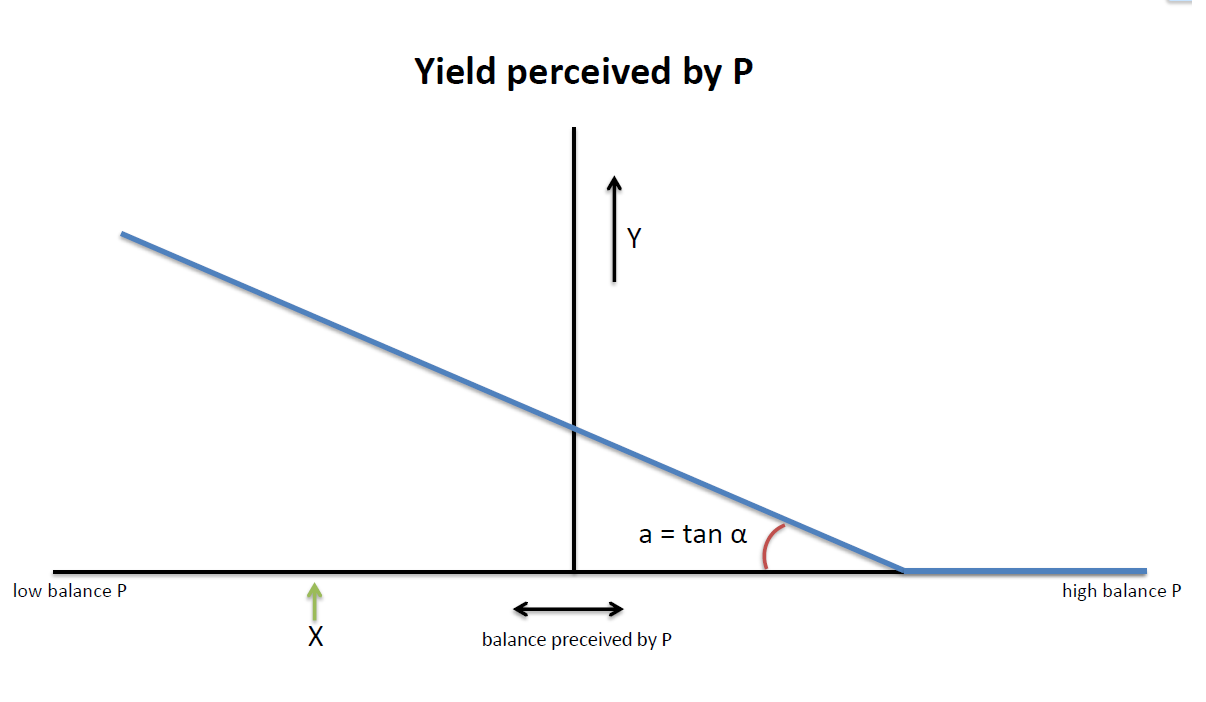
\includegraphics[scale=0.4]{YieldCurves/yieldcurve_P}
\caption{Yield curve, yield perceived by P.}
\end{figure}
\\
From the yield curve shown in figure 2.1 it is clear that when the account balance of P with Q gets higher the yield gets lower, but will never fall below 0. Once a high enough account balance would be reached that would result in a negative yield, the yield is set to 0. The yield curve is not always a linear function. Different ways of calculating the yield can lead to different yield curves. This thesis makes use of a simplified version of the yield curve where a linear function is used.
\\
\\
The yield will be important to determine who will receive a good next. If P would for example want to maximize its profit P would only want to give away a good to someone generating the highest yield. Agents who are in debt with P and are not likely to pay off their debt are of less value to P. It would be a bad investment if P would give to these agents.
\\
\\
The yield curve can either be used to predict the course of the transactions or to see an equilibrium arise. When an equilibrium arises the yield of a good between two agents switches between two values. Both agents perceive the transactions with each other as the most valuable and will keep giving to each other. These agents have established a community with each other and this community will hold as long as the current condition do not change. 
\begin{figure}[h!]
\centering
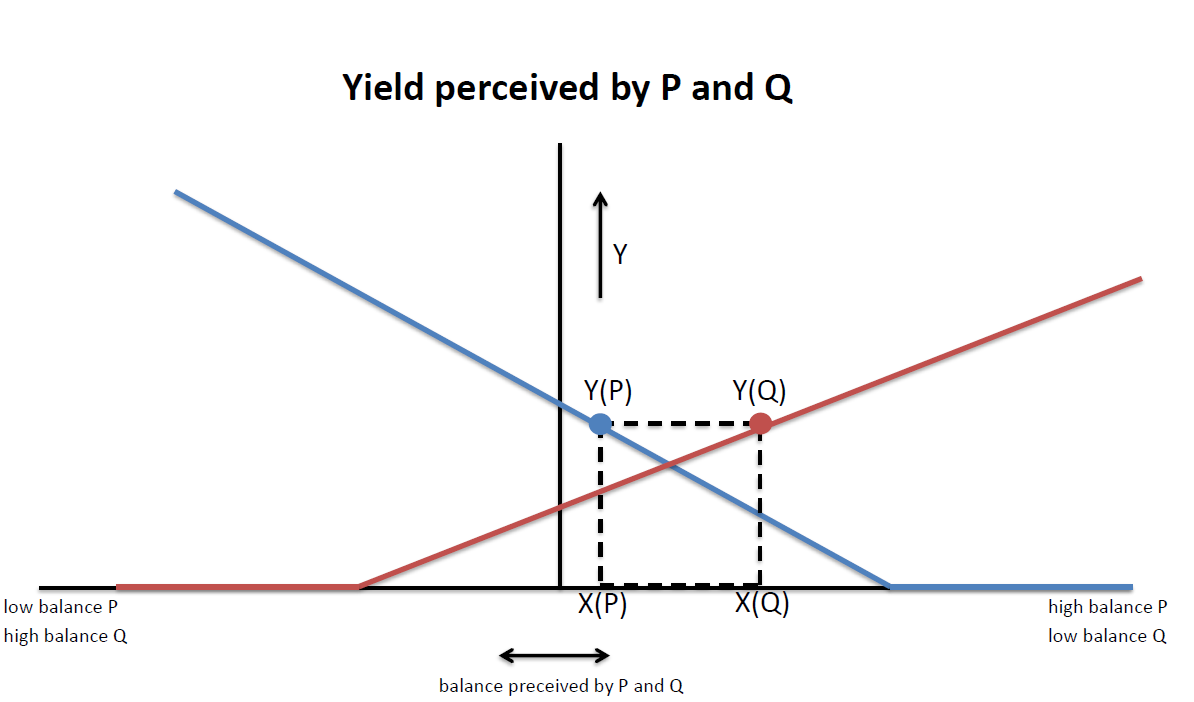
\includegraphics[scale=0.4]{YieldCurves/yieldcurve_PQ_equilibrium}
\caption{Equilibrium between P and Q.}
\end{figure}

\clearpage
\section{Research questions}
As explained earlier, in real life people seem to prefer under certain conditions to give to 'friends' than to strangers. When people only give to a certain number of people the transactions will only take place within a small subgroup of the whole population. When this happens a community arises of people who prefer to give to each other. This is called the community effect. This has led to the following research question:
\\
\\
\textit{In a Giving Game simulation will transactions eventually take place within a limited subgroup of the entire population?}
\\
\\
Another possible behaviour that can be seen in an environment with an economy of giving is the stabilization of transactions. Even if no community effect emerges the transactions can still fall into a repeating sequence. The behaviour will be very predictable and the transactions are executed in a certain order. When the sequence of transactions is not random the transactions have stabilized. This has led to the second research question:
\\
\\
\textit{In a Giving Game simulation will we see a repeating sequence of transactions or will the transaction sequence look random?}

To be able to answer these research questions the method explained in the next section will be used.

\section{Method}
To research the behaviour of agents within an economy of giving a simulation program will be build to simulate this behaviour. The simulation program will use the giving game mentioned in the previous sections for the simulations. The giving game for the simulations is further explained in the next chapter. The simulator uses three different selection rules. For every transaction the selection rule decides which agent will receive a good. Multiple simulations will be run to examine the behaviour when these selection rules are used. Different scenarios will therefore be developed for each selection rule where each scenario uses different parameters, for example different goods or different account balances at the start of the simulation. To be certain that the simulation program runs properly very basic scenarios will be developed to test this. The developed scenarios are explained in chapter 5. 

A simulation program has been chosen instead of a theoretical research, because it allows a better representation of a real life giving environment. With the simulation program multiple different scenarios can be tested more easily and eventually lead to a wide variety of results that can be used to understand and explain the behaviour of people within a giving environment.


\chapter{Design}
For this thesis the giving environment consists of a fixed amount of agents and a fixed amount of goods. For every simulation the number of agents and number of goods can be changed, but during the simulation no agents or goods are added or removed. Every agent keeps track of their own account balance and transaction values in relation to every other agent. The agents don’t know anything about each other, they operate completely independent.

There are two types of goods, ‘sustainable’ and ‘perishable’ goods. ‘Sustainable’ goods are goods that will exist for eternity. ‘Perishable’ goods are goods that perish after a certain amount of transactions. Every ‘perishable’ good has a producer. The producer is also an agent in the environment so the producer also participates in transactions of other goods. The producer reproduces its ‘perishable’ good after a certain amount of time the good has perished. The value of a good is valued differently by each agent, but this value does not change during the simulation. For the experiments in this thesis the agents are not able to hold on to a good for a certain amount of time. This is a variant which can be used in further research. Holding on to a good will be explained further in the last chapter. At the start of the giving game the goods can either be divided randomly over the agents or are divided by hand. The agents who start with the perishable goods are assigned to be the producers.

The transactions can be executed in two different ways. The transactions can be executed one by one which is a more game theory based approach. A more realistic approach is that the transactions are executed simultaneously, this way agents don’t have to wait for each other before they can give away their good. 

The emergence of a community effect is determined by the amount of transactions each agent is part of. When more than one good is used in the environment there can emerge multiple communities. That is why every good is looked at independently. Every agent keeps track of their own transactions and how much they have traded each good. If for example two agents hold 100 percent of the transactions of good A and two other agents hold 100 percent of the transactions of good B then two separate communities of size two have emerged. There can be concluded that the community effect exists for this scenario. If this time two agents hold 50 percent of the transactions of good A and good B and two other agents also hold 50 percent of the transactions of good A and good B than this means that one community has emerged with a size of four. There can also be concluded that a community effect exist in this scenario. A community effect can exists as long as the size of the subgroup is smaller than the total amount of agents in the environment and 100 percent of the transactions of one or more goods takes place inside this subgroup. This means that even if an agent holds a smaller percentage of the transactions this agent can still be part of the community as long as the previous stated rules apply.

The stabilization of the transactions in the environment can be determined by predicting future transactions. If multiple transactions in a row can be predicted or if a pattern is clearly visible then one may conclude that the transactions have stabilized. The emergence of a community does not mean that the transactions are executed in a repeating sequence. Even in a community the transactions can be executed randomly.


\section{Paramaters}
The following parameters will be used in the environment of the giving game for the experiments.

\begin{description}
\item[N:] The number of agents used in the simulation
\item[M:] The number of goods used in the simulation
\item[Perish period:] The perish period is the amount of transactions it takes before a good perishes. For sustainable goods the perish period is 0, because sustainable goods exist forever. For perishable goods the perish period is greater than 0. For example, when a good has a perish period of 3 then this good can be given away 3 times before it perishes. The perish period is a natural number greater than or equal to 0.
\item[Production delay:] The production delay is the time between the perish of a good and its reproduction. The time until the production is decreased by one after every iteration over all agents who are currently holding a good. The production delay is a natural number greater than or equal to 0.
\item[Nominal value:] The nominal value is an indication of how much a good is worth. The nominal value does not change during the giving game. Every agent perceives the nominal value of a good differently. Agent P could value good G more than agent Q for example. The nominal value is a natural number greater than or equal to 0.
\item[Like factor:] The like factor is a real number between 0 and 1 which defines how much agent P likes agent Q. The lower the number the more P likes Q and the more likely it is that P will give to Q. The like factor does not change during the giving game. 
\item[Selection rule:] The selection rule is an algorithm that decides/calculates the next agent(s) to receive a good.

\end{description}

\section{Selection rules}
For every transaction the selection rule decides which agent will receive a good. This decision is based on different parameters of the giving game. These selection rules simulate multiple real world scenarios for example: choosing the agent based on maximizing the profit (goodwill rule).

\subsection{Random rule}
The random rule is the most basic rule for the giving game. The agent who will receive the good during the transaction is chosen randomly. The random rule simulates an environment where the agents do not care about the value of the goods and do not care about who will receive the goods. The \textit{like factor} is therefore 0 for every agent pair. This rule is mostly used to see if the giving game environment behaves as it should.

\subsection{Balance rule}
A more advanced selection rule is the balance rule. The agent who will receive the good during the transaction is selected based on the balance between the giving agent P and the receiving agent Q. Agent P chooses agent Q if P has the highest balance with Q. If P has the same highest balance with multiple agents then the receiving agent is chosen randomly between these agents. The balance rule simulates an environment where each agent only gives to the agent from who they have received the most. Agent P tries to maximize the number of goods he receives. The balance in this case can be calculated as follows: 
\\
\\
\textit{Balance of P with Q = Number of goods received from Q – Number of goods given to Q} \\
This calculation of the balance is different from the calculation of the balance for the yield curve, but the following rule still applies:\\
\textit{Balance of P with Q = - (balance of Q with P)}

\subsection{Goodwill rule}
The goodwill rule is a more realistic rule. The agent is chosen based on the value of the transaction (the yield) between P and Q perceived by P. Only the agent where the yield is the highest is chosen as the receiving agent. If multiple agent pairs have the same yield the receiving agent is chosen randomly between these agents. Every time P gives good G to Q the value of the transaction of good G (the yield) decreases. As long as Q does not give good G to P, P loses interest in giving good G to Q. Eventually P will stop giving to Q, because P does not expect that Q will ever pay of his debt. The like factor as explained earlier defines how many transactions P can tolerate without getting anything in return from Q. For the goodwill rule the like factor can be set by the user or can be created randomly. The goodwill rule simulates an environment where every agent tries to maximize its profit. Agents who are in debt will less likely receive a good, they are not worth investing in. The yield curve would look like the yield curve in figure 3.1.\\
\begin{figure}[h!]
\centering
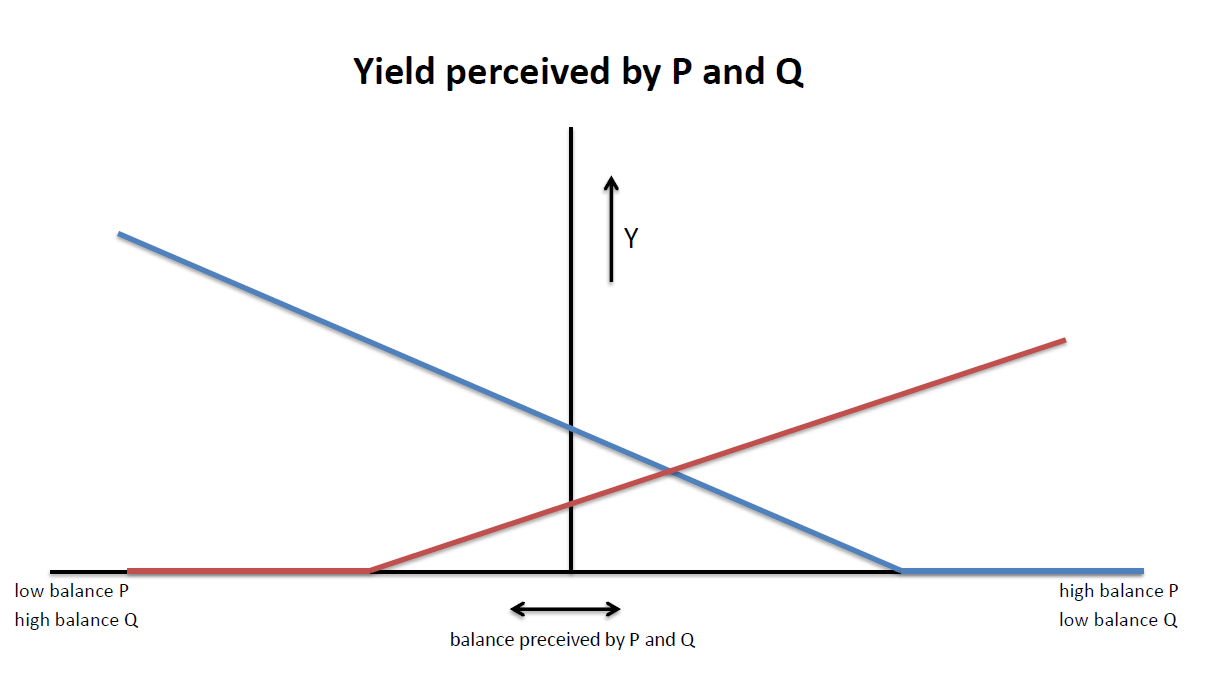
\includegraphics[scale=0.4]{YieldCurves/yieldcurve_PQ} 
\caption{Yield curve, yield perceived by P and Q}
\end{figure}
\\
The steeper the slope for YP the less tolerant P is. In this case the balance is calculated as explained before.
\\
\\
The expectation to receive something in return of a gift actually transforms that gift into an investment (with a certain likelihood to receive any gains in the future). The goodwill rule can be seen as a representation of an environment where people invest and all agents try to maximize profit they can get from such investment. A bad investment is looked down upon and in the future an investment in the same person will most likely not happen.

\section{Simulation model}
For the previously explained giving game a simulator will be created that can simulate different scenarios using the parameters and selection rules. The flow chart in figure 3.2 shows the actions that are executed to simulate the giving game. The technical side of the simulator will be explained in the next chapter. 
\begin{figure}[h!]
\centering
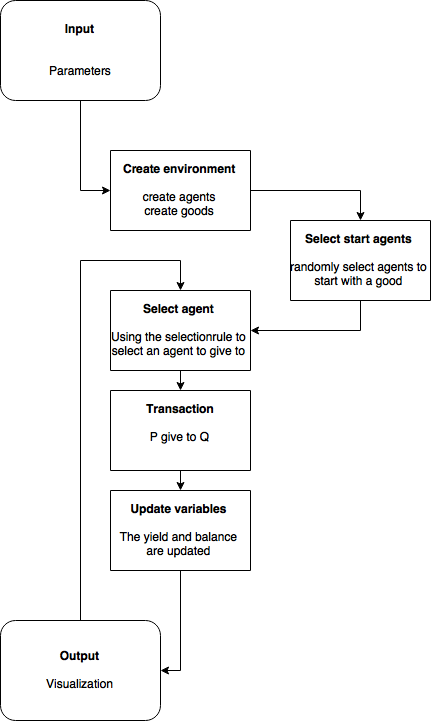
\includegraphics[scale=0.6]{FlowChart/FlowChart}
\caption{Flow chart of the simulation model.}
\end{figure}




\chapter{Implementation}
In this chapter the implementation of the simulator that will be used to simulate different scenarios for the giving game will be discussed. The simulation program is able to execute multiple tasks and accepts different user input to simulate multiple scenarios. The simulation program provides a visualization of the data that is produced during the simulation and a visualization of the course of the transactions. The whole program is created with \textit{Python} and uses multiple \textit{Python} modules, packages and frameworks. It can be run on a desktop with any operating system as long as the required \textit{Python} packages and frameworks are installed. 

\section{Back-end}
The back end consists of multiple components which together create an environment that simulates a giving economy where agents give and receive goods. This section will explain these components briefly and how they work together. The simulation program consists mostly of object oriented code, therefore classes are used to define some of the components.

\subsection{Agents}
Every agent is defined by the \textit{Agent} class. Every agent can be identified by an \textit{ID}. This \textit{ID} is an integer number greater than or equal to 0. Every agent keeps track of their own account balances, yield values, like factors and nominal values. The \textit{Agent} class is able to hold this data in the form of a \textit{Python} lists. The ID of every agent is used for these data lists to find the corresponding information about that agent. The agents only hold data of their own relations with the other agents and the goods, they don't hold data of anything else about the environment. The following information is stored in the memory of each agent:
\begin{itemize}
\item The amount of goods given and received to and from each agent.
\item The amount of times each good has been given and received by the agent.
\item The like factors in relation to the other agents.
\item The account balance with the other agents.
\item The nominal value of each good perceived by the agent.
\end{itemize}

\subsection{Goods}
Every good is defined by the Good class. Every good can be identified by an \textit{ID}. This \textit{ID} is an integer number greater than or equal to 0. This \textit{ID} can be used by the textit{Agent} class as an index for the python lists that hold information about this good. Goods have a 'life' which defines how many times this good can be traded. For every transaction of a good the life of that good is decreased by 1. Once the life of a good reaches 0 it is removed from the environment. Every good has a variable called the 'time\_until\_production' which defines the time until a good is reproduced. A good is reproduced and added back into the environment once the 'time\_until\_production' reaches zero. For every transaction in the environment the time until the production is decreased by 1.

\subsection{Selection rules}

\subsubsection{Random rule}
A random natural number is generated with the \textit{random} module from \textit{Python} with a different seed every time. The generated number is the \textit{ID} for the agent who should receive the good. Once the agent has been selected the transaction can proceed.

\subsubsection{Balance rule}
The balance rule finds for P the agent who P has the highest balance with. When P has the same balance with multiple agents the balance rule randomly selects one of these agents. The result is the \textit{ID} for the agent who should receive the good. Once the agent has been selected the transaction can proceed. After every transaction the account balance is updated for every agent who participated in the transaction.

\subsubsection{Goodwill rule}
The goodwill rule finds for P the agent who P has the highest yield with. When P has the same yield with multiple agents the goodwill rule randomly selects one of these agents. The result is the \textit{ID} for the agent who should receive the good. Once the agent has been selected the transaction can proceed. After every transaction the account balances are updated with the yield for every agent participated in the transaction. With the new account balance the yield is updated for the goods used in the transaction.

\subsection{Environment}
Every simulation has an environment where everything happens. The environment is defined by the Environment class. The environment holds all the information for the simulation to run properly. The environment holds N number of agents and M number of goods and are stored in two \textit{Python} lists. The environment keeps track of all the input parameters and output data.

\subsection{The Simulation}
The simulation is run by first creating the environment. First the agents and the goods are created by calling their corresponding classes. After the goods have been created the agents are notified, their perception of the nominal values of these goods and the yield values for the first transactions are updated. The goods are either randomly assigned to the agents or chosen by the user. The agents who start with a perishable good are assigned to be the producer of this good. This means that when a good is reproduced by the environment the producer is the first one to get this good. This is not seen as a transaction, the producer acts as if he is the one creating the good. Once the whole environment is created a never ending loop (unless the user pauses or stops the simulation) is initiated and the appropriate actions are executed as shown in chapter 3.3.


\section{Front-end}
The front end provides the interface between the user and the back end. With this interface the user is able to put data into the simulation to simulate different scenarios. The interface is able to visualize the responses of the back end to analyse the resulting data during the simulation. The front end is written in \textit{Python} using the \textit{PyQt4} framework. Graphs are drawn using \textit{matplotlib} and the visualization of the transactions as shown in figure 4.2 is written using the \textit{VisPy} framework. For the explanation of the use of the interface the use should consult the user manual which can be found in appendix A.

\subsubsection{Input}
The user is able to set the following parameters:

\begin{description}
\item[N:] An integer number that defines the number of agents.
\item[M:] An integer number that defines the number of goods.
\item[Perish period:] An integer number that can be set for every good.
\item[Production delay:] An integer number that can be set for every good.
\item[Selection rule:] The user can choose between the given selection rules (random rule, balance rule and goodwill rule). 
\item[Nominal value:] The user is able to choose if every agent perceives the value of a good differently or not. If the user wants to have a different value of the good for every agent the user can add a \textit{xls} or a\textit{xlsx} file with the nominal values as shown in figure 4.1.
\item[Like factor:] The user is able to choose between setting like factors by hand or to randomly create the like factors. If the user wants to add predefined like factors the user can add a \textit{xls} or a\textit{xlsx} file with the like factors as shown in figure 4.2.
\item[Balance:] The user is able to set the balance at the start of the simulation at 0 or to set different balances for every agent pair by adding a \textit{xls} or a\textit{xlsx} file as shown in figure 4.3. Because of how the account balance is defined the user only has to fill half of a matrix.
\end{description}

\begin{figure}[h]
\centering
\begin{minipage}{.5\textwidth}
\centering
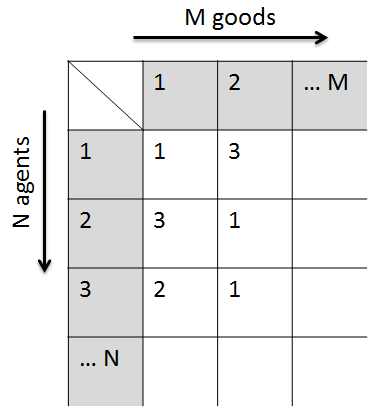
\includegraphics[width=.4\linewidth]{Matrices/Nominal_values}
\captionof{figure}{Matrix format for the nominal values}
\end{minipage}%
\begin{minipage}{.6\textwidth}
\centering
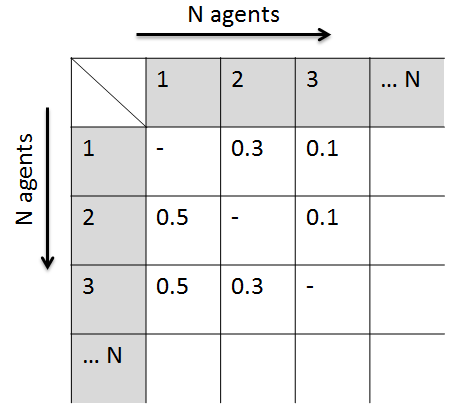
\includegraphics[width=.4\linewidth]{Matrices/Like_factors}
\captionof{figure}{Matrix format for the like factors.}
\label{fig:test2}
\end{minipage}
\begin{minipage}{.6\textwidth}
\centering
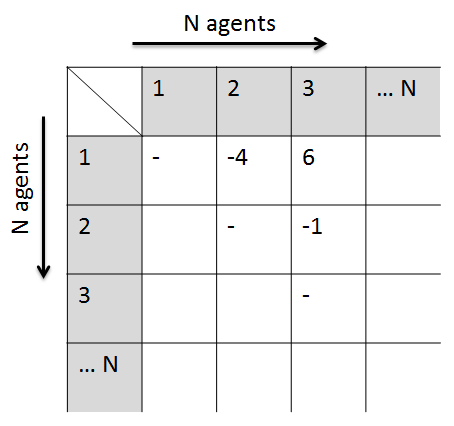
\includegraphics[width=.4\linewidth]{Matrices/Account_balance}
\captionof{figure}{Matrix format for the account balances.}
\label{fig:test3}
\end{minipage}
\end{figure}


During the simulation the user is able to adjust the following variables:

\begin{description}
\item[Subgroup size:] The user is able to change the size of a subgroup to see how many agents hold 100 percent of the transactions. The default value is 2.
\item[Reset community percentage:] The user is able to reset the number transactions that has been executed and the number of times each agent has contributed to a transaction. This allows the user to see if from a certain point in the simulation the transactions only take place within a subgroup.
\item[Delay:] The user is able to set a delay which increases the time between each transaction. The user can set a maximum delay of 1 second. 
\item[Pause:] The user is able to pause the simulation at any time. The simulation will continue once the user chooses so.
\end{description}


\subsubsection{Output}
The output data is visualized so that the user is able to analyse and get results without doing any calculations. The simulator is able to give the following output:
\begin{itemize}
\item Show the amount of goods given and received for each agent.
\item Show the yield curve between every agent pair.
\item Show the amount of transactions
\item Show percentages of how many times a certain good has been traded by an agent (Figure 4.4).
\item Show the visualization of the course of the transactions with a colour indication that shows the percentage of transactions each agent participated in (Figure 4.5). 
\item Show every transaction, production and delay in production (Figure 4.6).
\item Show the community percentage, the percentage of transactions that take place in a subgroup with the set subgroup size.
\end{itemize}

The output is updated after every transaction. All the data can be saved and used in the future for another simulation.

\begin{figure}[h]
\centering
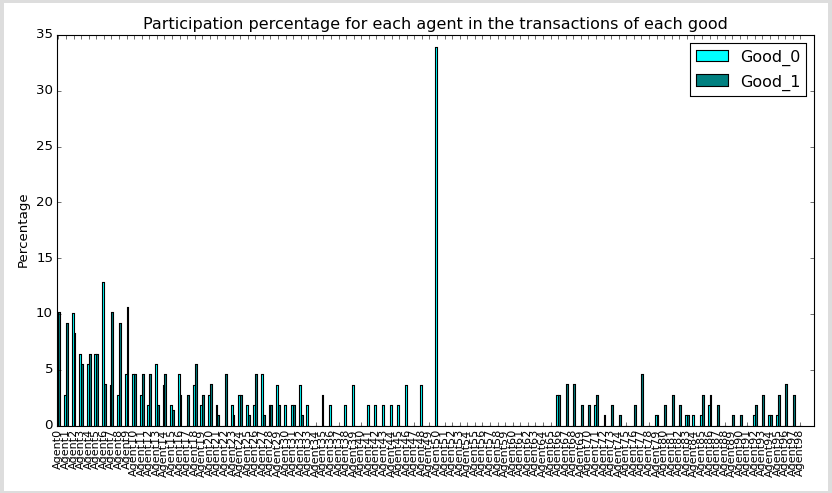
\includegraphics[scale=0.4]{Simulation2_figures/Distribution}
\caption{Transaction percentage of each good by each agent}
\end{figure}
\clearpage
\begin{figure}
\centering
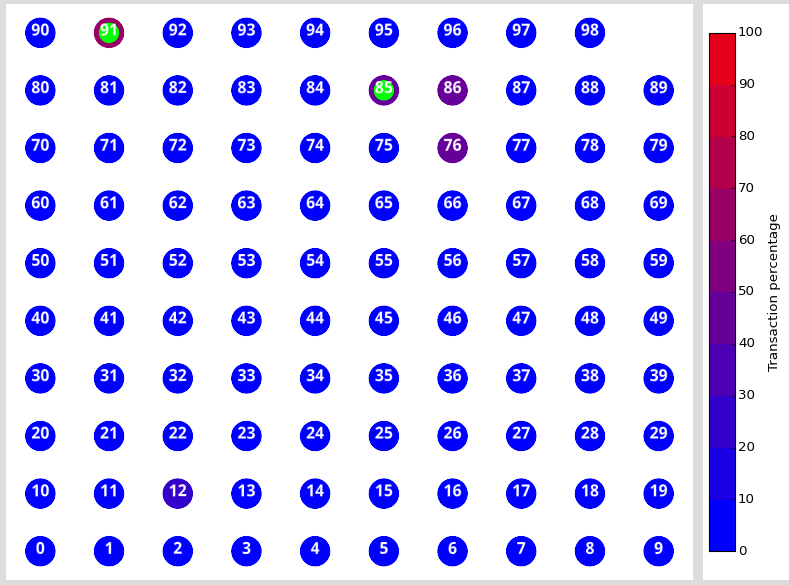
\includegraphics[scale=0.4]{Simulation2_figures/Visualization}
\caption{Visualization of the course of the transactions}
\end{figure}

\begin{figure}
\centering
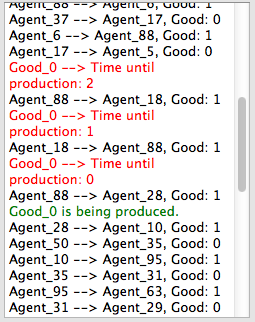
\includegraphics[scale=0.4]{Simulation2_figures/Transactions}
\caption{Executed Transactions}
\end{figure}


\chapter{Scenarios}
For every selection rule multiple scenarios have been created where the scenarios define the starting parameters used for the simulations of the selection rules. This chapter will explain the scenarios used in the experiments. For every scenario 99 agents will be used. 99 agents is large enough to have as much variety in the parameters as possible but still be able to clearly see any changes in the visualisation. 

\section{Basic Scenarios}
For every selection rule the behaviour is tested in the most basic environment. These scenarios will be used to see if the selection rules are implemented correctly.

\subsubsection{Basic scenario 1, sustainable (BS\_S):}
Parameters:
\begin{itemize}
\item 99 agents
\item 1 sustainable good with a nominal value of 1, perish time of 0, perish delay of 0
\end{itemize}
\subsubsection{Basic scenario 2, perishable (BS\_P):}
Parameters:
\begin{itemize}
\item 99 agents
\item 1 perishable good with a nominal value of 1, perish time of 1, perish delay of 1
\end{itemize}
In case of the goodwill rule where the like factor is used for the selection of an agent the like factor is set to 0.5 for every agent. In the most basic environment every agent is equal and has no specific relations with other agents.

\section{Random rule}
The following scenarios are used to see if the agents behave as predicted with the random rule. Any irregularities in the behaviour will be analysed and can be used in decisions for further experiments. The nominal value does not have to be set, because the nominal values of the goods are not used in the selection of an agent.
\subsubsection{Scenario 1, sustainable (RR\_S):}
Parameters:
\begin{itemize}
\item 99 agents
\item 3 sustainable goods
\end{itemize}
\subsubsection{Scenario 2, perishable (RR\_P):}
Parameters:
\begin{itemize}
\item 99 agents
\item 3 perishable goods with a perish time of [1,2,3], perish delay of [1,2,3]
\end{itemize}
The number of goods is not a fixed number, during the experiments the number of goods will differ to see if this affects the results.

\subsubsection{Hypothesis}
It is expected that no community effect will arise, neither will the simulation stabilize even though a machine is pseudorandom. The transactions will eventually be equally distributed over all the agents. For perishable goods this distribution will be in favour of the producers, because they will be able to give away their good more than others.

\section{Balance rule}
The scenarios for the balance rule will be used to see how people will behave when they care about how many goods they give and receive but do not have any relationship with other agents. The nominal value does not have to be set, because the nominal values of the goods are not used in the selection of an agent.
\subsubsection{Scenario 1, sustainable (BR\_S):}
Parameters:
\begin{itemize}
\item 100 agents
\item 3 sustainable goods
\end{itemize}
\subsubsection{Scenario 2, perishable (BR\_P):}
Parameters:
\begin{itemize}
\item 100 agents
\item 3 perishable goods with a perish time of [1,2,3], perish delay of [1,2,3]
\end{itemize}
The amount of goods is not a fixed amount, during the experiments the amount of goods will differ to see if this affects the results.

\subsubsection{Hypothesis}
The expectations are that a community effect will arise with a subgroup consisting of a few agents. The size of this subgroup is based on the type of goods and the amount of goods. All sustainable goods will eventually be traded only between two agents, because these two agents have the highest balance with each other. Every perishable good has a producer, these producers will also be part of a subgroup. If these producers only give each other their goods then the subgroup size will be as large as the amount of producers. If the producers each give to another agent then multiple subgroups will arise with a size of two. It is expected that the maximum size of a subgroup will be the number of producers plus one non-producer who trades with the producers.

\section{Goodwill rule}
For the goodwill rule all parameters can affect the results. The following parameters define the scenarios.
\subsubsection{Like factors}
\begin{description}
\item[L1] 1/3 of the population has a like factor of 1, 1/3 of the population has a like factor of 0.5 and 1/3 of the population has a like factor of 0.1. This means that every agent has a different relationship with every third of the population. These three groups have been chosen in order to better observe the difference in behaviour.
\item[L2] 47 agents have a like factor of 1, 47 agents have a like factor of 0.5 and 5 of the agents have a like factor of 0.1. This means that only a small group of agents is liked by all other agents.
\end{description}
\subsubsection{Balances}
\begin{description}
\item[B1] At the start of the simulation all account balances are set to 0.
\item[B2] At the start of the simulation all account balances are randomly set. The account balance for every agent will be a natural number between -9 and 9. These values have been chosen to simulate an environment where some agents have really high debts and others don't.
\end{description}
\subsubsection{Nominal values}
\begin{description}
\item[N1] The nominal values of every good are the same for every agent.
\item[N2] Every third of the agents perceives the nominal values of all goods differently. Just like the like factors, the population is divided into 3 groups, where every group perceives the value of the goods differently. The first group perceives the nominal value of the good as 1, the second group as 2 and the third group as 3. For every additional good the nominal value of the next good is increased by 1. The groups are the same groups as with L1. These values have been chosen to have three very different groups of agents and as much variety in nominal values. The difference between the nominal values is limited to prevent unrealistic high yield values.
\end{description} 
The combination of these parameters will form different scenarios. Every combination will be tested unless previous experiments show that one of the parameters does not affect the result. The scenarios are based on the idea of having a population where people have different relationships with each other and value goods differently. That’s why the population is split into 3 groups to have groups that are completely different from each other. The following scenarios will be used during the experiments.
The first scenarios are scenarios where the balance is zero.

\begin{description}
\item[GR\_L1B1N1], Goodwill rule using L1, B1 and N1 as input.
\item[GR\_L1B1N2], Goodwill rule using L1, B1 and N2 as input.
\item[GR\_L2B1N1], Goodwill rule using L2, B1 and N1 as input.
\item[GR\_L2B1N2], Goodwill rule using L2, B1 and N2 as input.
\end{description}
After these scenarios B2 will be used for the balances.
\begin{description}
\item[GR\_L1B2N1], Goodwill rule using L1, B2 and N1 as input.
\item[GR\_L1B2N2], Goodwill rule using L2, B2 and N2 as input.
\item[GR\_L2B2N1], Goodwill rule using L1, B2 and N1 as input.
\item[GR\_L2B2N2], Goodwill rule using L2, B2 and N2 as input.
\end{description}

\subsubsection{Hypothesis}
Expectations are that for all scenarios a community effect will arise with one or more subgroups consisting of agent with a low like factor. A low like factor would mean that the agent like each other, so it would be logically to assume that these agent will trade more with each other than with agents who are not liked. When B2 is used instead of B1 or N2 instead of N1 the results will most likely vary a lot more, because of the varying starting values. Assuming agents prefer agents with a low like factor using L2 will most likely lead to smaller communities or a longer time before a community arises.



\chapter{Results}
The scenarios mentioned in the previous chapter are used in the simulator. For every scenario except for the basic scenarios multiple experiments have been performed using a different amount of goods. The amount of goods used for each scenario are 1, 2, 3, 5, 20, 50, and 99.

\section{Random rule}

\subsection{Results}

\subsubsection{BS\_S}
No community effect arose and the transaction also did not stabilize. The transactions are still completely random. After 100000 transactions every agent participated in 0.9-1.1 percent of the transactions. More transactions will lead to more evenly distributed transactions.

\subsubsection{BS\_P}
The producer participated in 100 percent of the transactions, because after each time the producer gives away his good it perishes. The other 50 percent of the transactions is distributed over the other 98 agents. Each agent participated in approximately 1 percent of the transactions. No community effect arose and the transactions did not stabilize.

\subsubsection{RR\_S}
The results are similar to the results from BS\_S. No community arose, neither did the transactions stabilize. All the transactions of each good were evenly distributed over all agents. 

\subsubsection{RR\_P}
The results are similar to the results from RR\_N2. No community arose, neither did the transactions stabilize. Good\_1 is the good with the lowest perish period and the lowest production time. The producer of this good participated in 100 percent of the transactions of this good. The producer of Good\_2 participated in approximately 50 percent of the transactions of Good\_2, because the perish period of Good\_2 is twice the amount of the perish period of Good\_1. The producer of Good\_3 participated in approximately 35 percent of the transactions of Good\_3, because the perish period of Good\_3 is three times the amount of the perish period of Good\_1. The higher the perish period the more the goods look like a sustainable good and the more the transactions are evenly distributed over all agents.\\
\begin{figure}[h!]
\centering
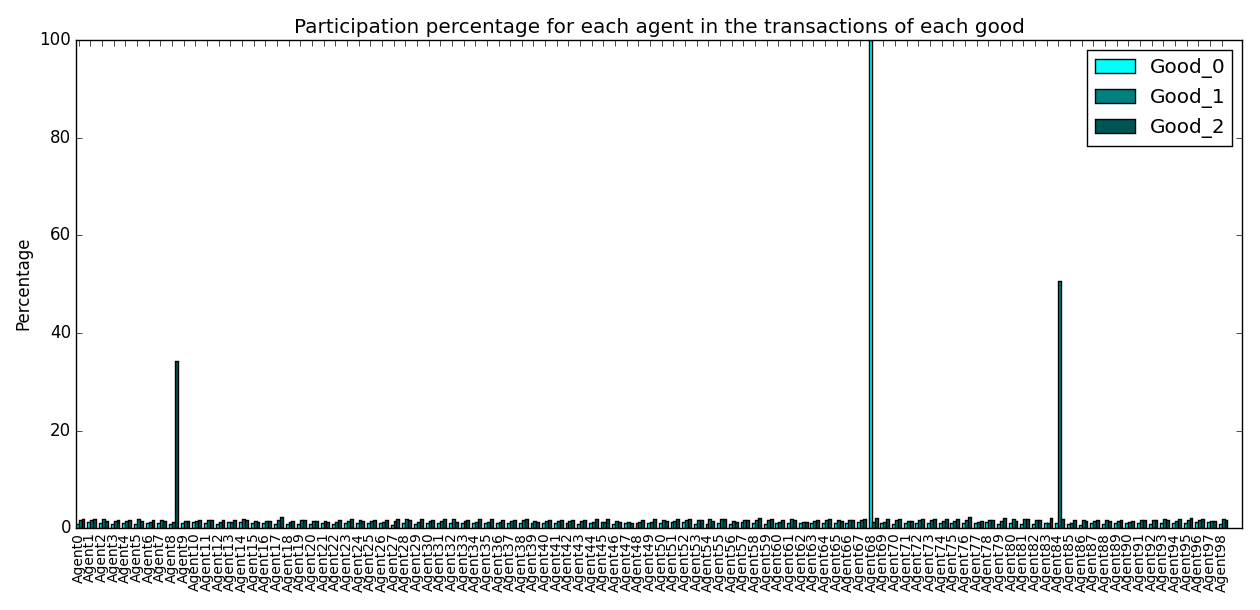
\includegraphics[scale=0.4]{Simulation_figures/RR_P/Figure1_20k}
\caption{Transaction percentages for RR\_P.}
\end{figure}

\subsection{Recap}
The scenarios BS\_S and BS\_P have confirmed a correct implementation of the random rule, for every transaction the agents are randomly chosen. The scenarios RR\_S and RR\_P confirmed the hypothesis, no community effect and no repeating sequence of transactions has emerged. The simulation program can execute transactions correctly. More goods did not affect the results.

\section{Balance rule}
\subsection{Results}

\subsubsection{BS\_S}
Every time an agent receives a good the good is given back to the agent who gave the good. The moment P gives Q the good Q has the highest balance with P, because Q has received more from P than Q has given to P. This means that Q will give the good to P during the next transaction which means that all agents have the same balance with P again. Now P has to choose randomly who should receive the good next. No community arises, but the simulation is partially stabilized. It is partially stabilized because P will always get the good back after P has given it away. The only thing that is still random is the choice for P to who P should give to. \\
\begin{figure}[h!]
\centering
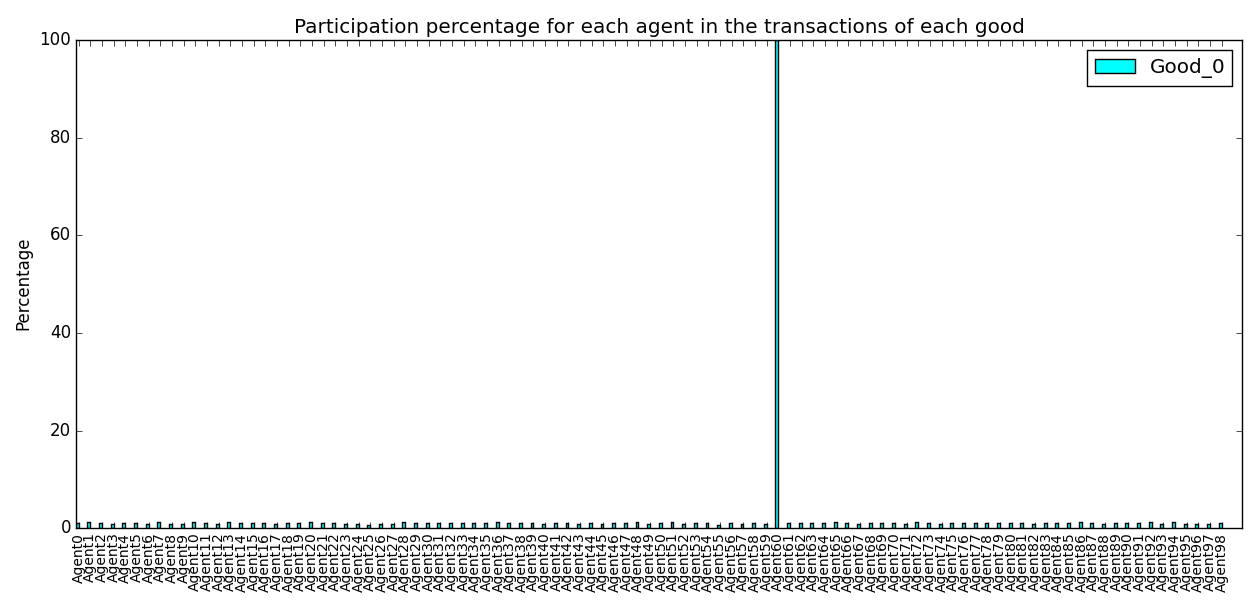
\includegraphics[scale=0.4]{Simulation_figures/BR_BS_S/Figure1_10k}
\caption{Transaction percentage for BS\_S.}
\end{figure}


\subsubsection{BS\_P}
The producer participated in 100 percent of the transactions, because after each time the producer give away its product it perishes. Each other agent participated in approximately 1 percent of the transactions. The moment the producer gives the good to let's say agent Q the balance of the producer with Q is now lower than the balance of the producer with all other agents. This means that the next transaction the producer will not give to Q but has to choose randomly between all the other 98 agents, because the balance of the producer with the other agents is equal to each other. The same happens after the next transactions, now the producer has to choose randomly between 97 agents. This goes on until 1 agent is left to choose from, at this point the choice is not random anymore, because only 1 agent is left. After this agent has received a good from the producer everyone is equal again and the whole process starts from the beginning. This leads to the conclusion that after every 98 transactions the next transaction can be predicted. No community effect arises, but the transactions are partially stabilized. \\
\begin{figure}[h!]
\centering
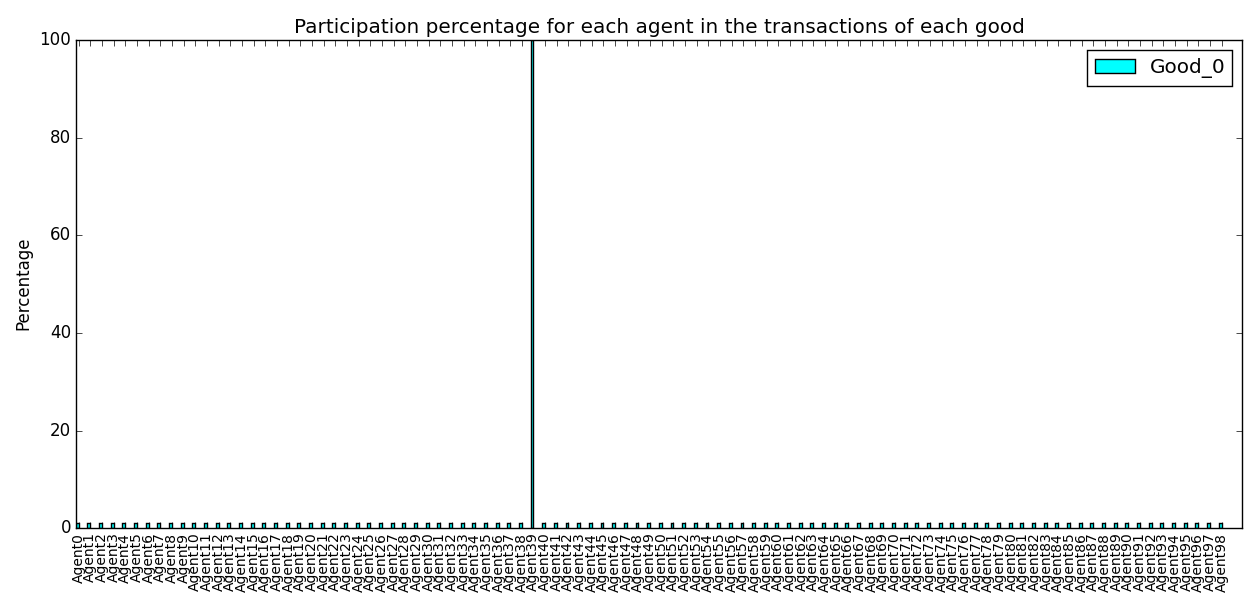
\includegraphics[scale=0.4]{Simulation_figures/BR_BS_P/Figure1_10k} 
\caption{Transaction percentages for BS\_P.}
\end{figure}


\subsubsection{BR\_S} 
The results are similar to the results from BS\_S where the goods are returned to the giving agent after each transaction. The only difference is that the agents who start with the goods at the start of the simulation participate in proportion more in transactions of each other’s goods than the other agents do as shown in figure 6.4. This happens when two agents who each start with a good trade their good for the good of the other. Both agents are now in possestion of a different good and can now give this good to someone else. \\
\begin{figure}[h!]
\centering
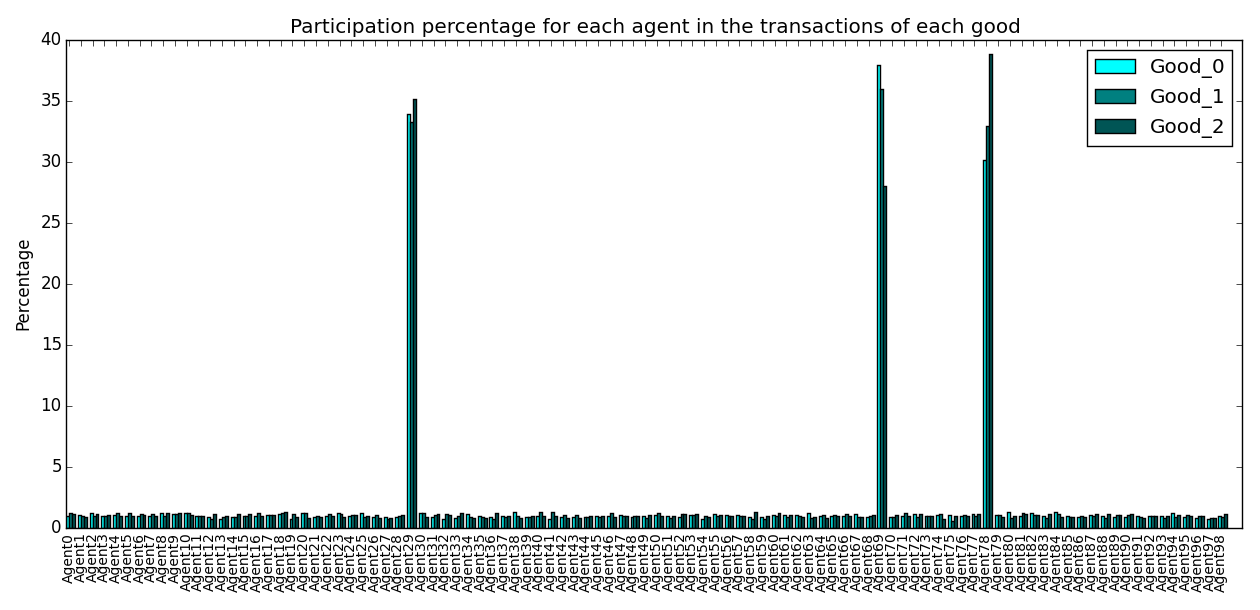
\includegraphics[scale=0.4]{Simulation_figures/BR_S/Figure1_30k}
\caption{Transaction percentages for BR\_S.}
\end{figure}
\newpage


\subsubsection{BR\_P}
When the perish period of a good is an even number the behaviour is equal to the behaviour of a sustainable good shown in BR\_S. When the perish period of a good is an odd number the good is also more traded with the other producers than with other agents, but the transactions with the other agents show the same behaviour as BS\_P. 
\begin{figure}[h!]
\centering
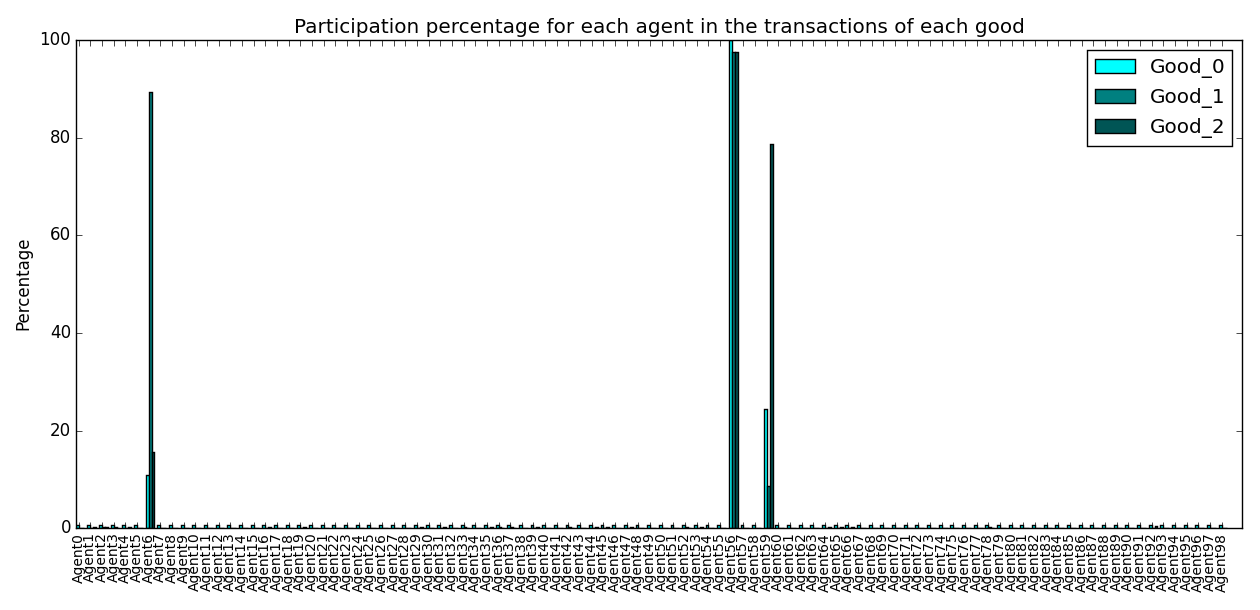
\includegraphics[scale=0.4]{Simulation_figures/BR_P/Figure1_10k}
\caption{Transaction percentage for BR\_P.}
\end{figure}

\subsection{Recap}
 The scenarios BR\_S and BR\_P show different behaviour than what was expected. No community effect arises, which in the end makes sense, because once a good is given it is immediatly returned. The same behaviour occured when more goods were used. The scenarios BS\_S and BS\_P have confirmed a correct implementation of the balance rule and show a correct calculation of the balances even though the expectations were different at first.


\section{Goodwill rule}
 The scenarios for the goodwill rule are split into two parts. The first part (B1) uses an account balance for the agents that start at 0. The second part (B2) uses an account balance for the agents that is randomly chosen and different for some agents at the start of the simulation. 
\subsubsection{BS\_S}
Immediately at the start of the simulation a community effect arises with a subgroup of size two. Where the subgroup arises depends on which agent starts with the good. If for example P would start with the good P would randomly choose an agent Q to give to, because at the start the yield is the same for everyone for this experiment. The moment agent P gives to agent Q, Q is in debt with P. This means that Q values the next transaction more with P. So Q will give to P during the next transaction. Now P values the transaction with Q more than with any other agent, so P gives back to Q. An equilibrium has emerged where the yield of the transactions for P with Q and Q with P will switch between the same two values.  

\subsubsection{BS\_P}
No community effect and no repeating sequence of transactions arises. At the beginning the yield is the same for everyone so the producer randomly selects an agent. Once the good is given away the good perishes. In the beginning the yields between the producer and the agents differs, so some transactions will not be at random. Eventually the yield between the producer and the agents will become 0, because the agents cannot give anything in return. From this point on the transactions are random again.
\begin{figure}[h!]
\centering
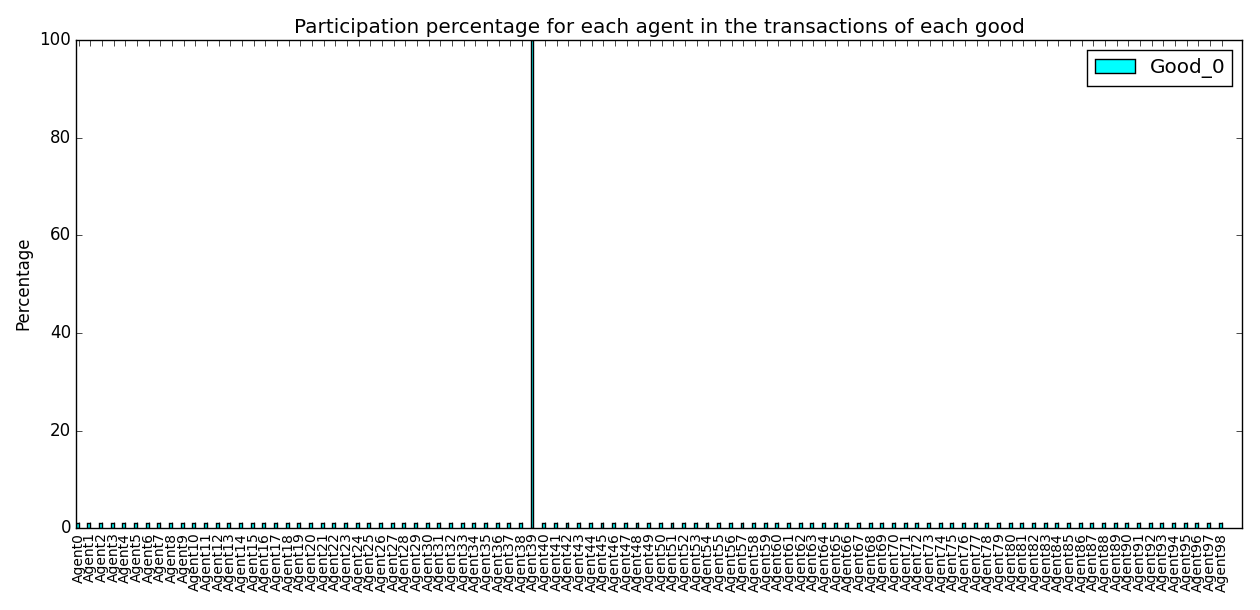
\includegraphics[scale=0.4]{Simulation2_figures/GR_BS_P/Figure1_4k}
\caption{Transaction percentage for BS\_P.}
\end{figure}

\subsubsection{GR\_L1B1N1}
Because all the balances are zero at the start and the nominal values are the same for every agent the yield of the first transaction is the same for everyone. The agent who first starts with the good randomly gives the good to another agent. From this point on the subgroup has emerged and the good will only be traded between two agents. Good\_0 is from the beginning only traded within a subgroup of size 2. When P gives to Q, Q is in debt with P and values giving to P more than giving to anyone else, the yield is the highest between Q and P. Q gives back to P and now the yield for P has become greater than the nominal value so P values the transaction with Q the most. An equilibrium just like with BS\_S has emerged. Changing the amount of goods did not change the results. Each good is only traded between 2 agents with a like factor of either 1, 0.5 or 0.1.
\\
\\
For the perishable goods the results are very different. With one perishable good and a perish period of 1 all experiments led to a community of the producer and all the agents with a like factor of 0.1 and 0.5 as shown in figure 6.7 Because the good perishes after it has been given away by the producer the agents who receive the good stay in debt with the producer. The producer therefore prefers the agents with a like factor of 0.1 and 0.5 over 1. \\
\begin{figure}[h!]
\centering
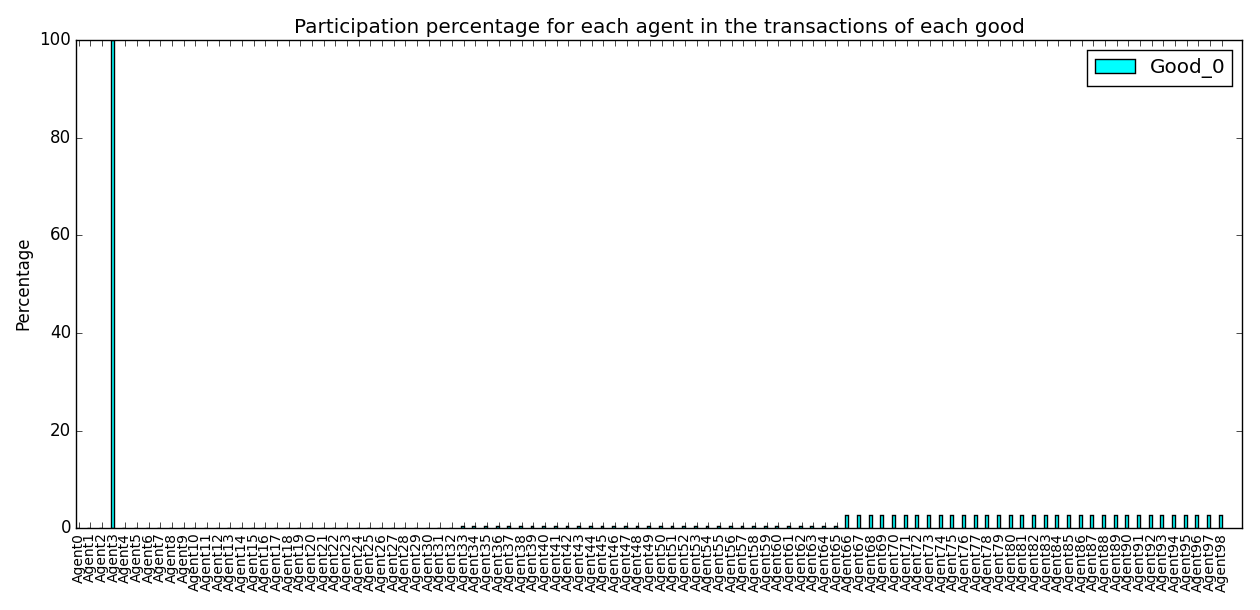
\includegraphics[scale=0.4]{Simulation_figures/GR_L1B1N1/1perishable_1-1_15k}
\caption{Transaction percentage for GR\_L1B1N1 with 1 perishable good.}
\end{figure}

When an odd number is used for the perish period the results are similar to the results shown in figure 6.7 but instead the producer only gives to agents with like factors 0.1. When an even number is used for the perish period the goods act as if they are sustainable and immediately are only traded within a subgroup of two agents with like factors of iether 1, 0.5 or 0.1. 

\subsubsection{GR\_L1B1N2}
In the beginning some goods are traded between different agents. This happens because after some transactions the yield is the same value as the nominal value of the good. This means that the yield is the same for some agents. The agent who is giving the good will have to choose randomly between these agents, which can lead to a transaction with a different agent. This happens for example between agents where their nominal value is a multiple of the other and the like factors are 1 and 0.5. After a few transactions the calculation of the yield with these values results in the same value as the nominal value of the good, thus an agent needs to be randomly selected again. This is a rare occurrence and eventually each good is only traded between two agents with either like factor of 1, 0.5 or 0.1, depending on which agent starts with the good. Changing the amount of goods did not affect the results.

For the perishable goods the results are the same as the results from GR\_L1B1N1. Changing the nominal value does not seem to affect the behaviour of perishable goods.
\subsubsection{GR\_L2B1N1}
The results are the same as the results from GR\_L1B1N1. Changing the size of the group with a like factor of 0.1 did not change anything. 
\subsubsection{GR\_L2B1N2}
The results are similar to the results from GR\_L1B1N2. Changing the size of the group with a like factor of 0.1 did not change anything. 

\clearpage
\subsubsection{GR\_L1B2N1}
Firstly the experiments with sustainable goods show in the beginning that the transactions are mostly divided over the agents with a like factor of 1 and 0.5. After the first 1000 transactions the transaction percentage is as shown in figure 6.8. \\
\begin{figure}[h!]
\centering
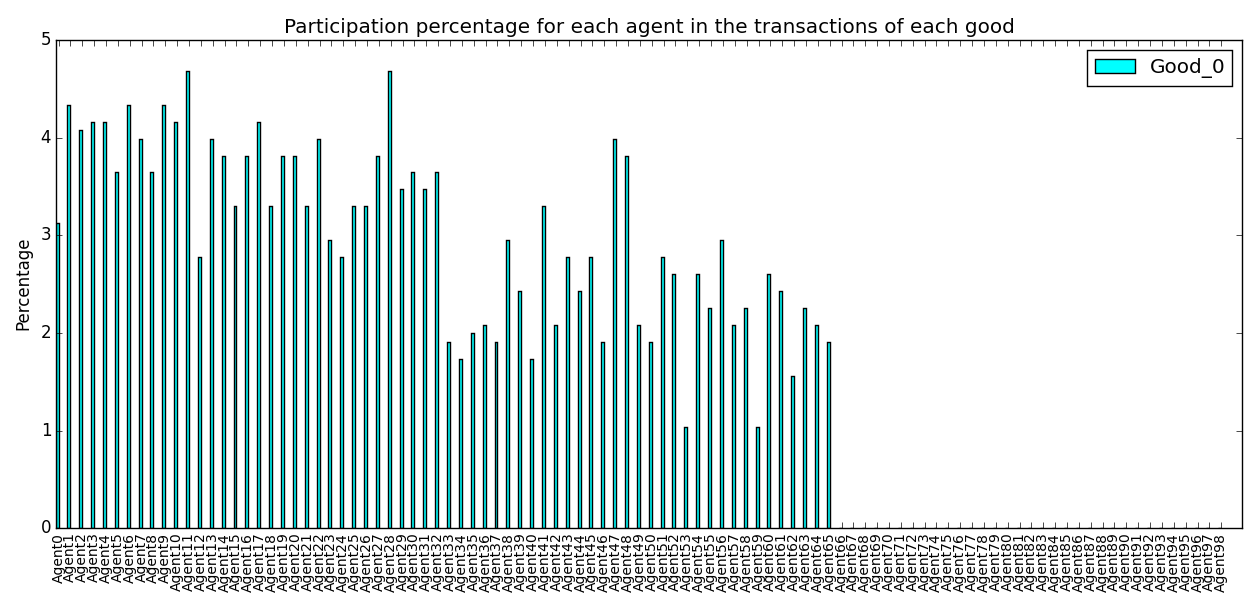
\includegraphics[scale=0.4]{Simulation2_figures/GR_L1B2N1/Figure1_1good_1k}
\caption{Transaction percentage for GR\_L1B2N1 with 1 sustainable good.}
\end{figure}
\\
After 4000 transactions a subgroup started to arise. Figure 6.9 shows the emergence of this subgroup and show that the agents with a like factor of 0.1 eventually also participate in some transactions. \\
\begin{figure}[h!]
\centering
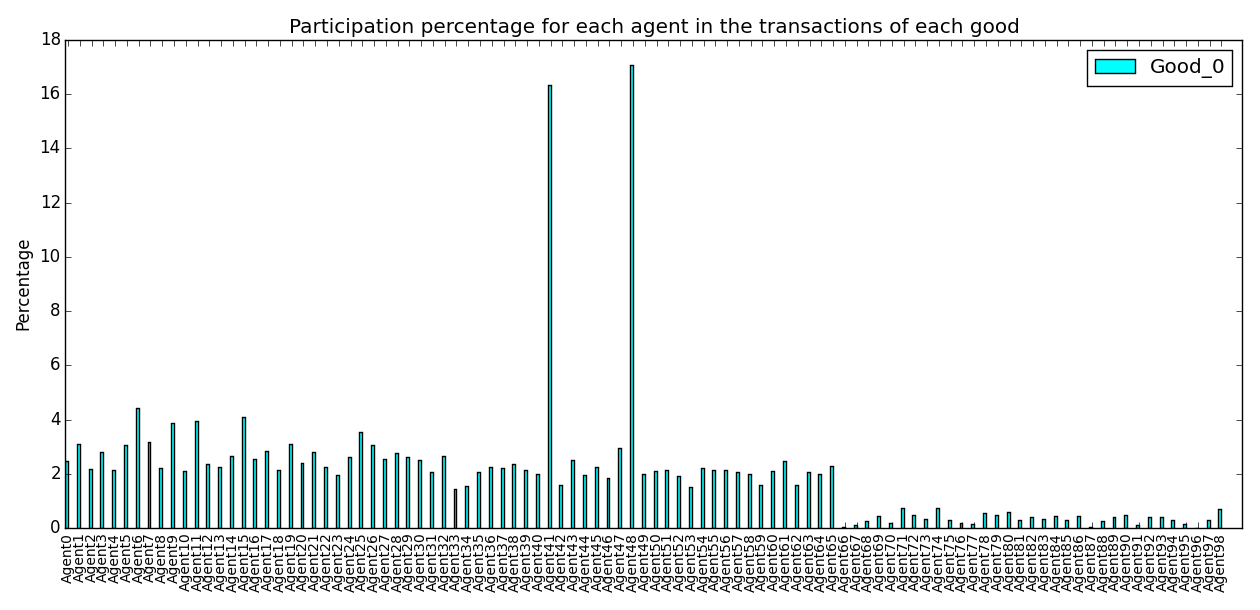
\includegraphics[scale=0.4]{Simulation2_figures/GR_L1B2N1/Figure2_1good_4k} 
\caption{Transaction percentage for GR\_L1B2N1 with 1 sustainable good.}
\end{figure}
\\
Every experiment with just one good led to a subgroup of agents with like factor 0.5 or 1. With just one good the good was only traded between 2 agents after 4000-5000 transactions. When more goods are used the results start to vary a lot more. Figure 6.10 shows what happens when more than one good is used. When more goods are used the goods sometimes fall into a subgroup for a short period of time. Eventually all goods are only traded between two agents. The goods are traded between multiple different subgroups until the highest equilibrium arises where the yield switches between the two highest possible values. The communities that arise only consists of agents with a like factor of 0.5 or 1 as shown in figure 6.11. \\
\begin{figure}[h!]
\centering
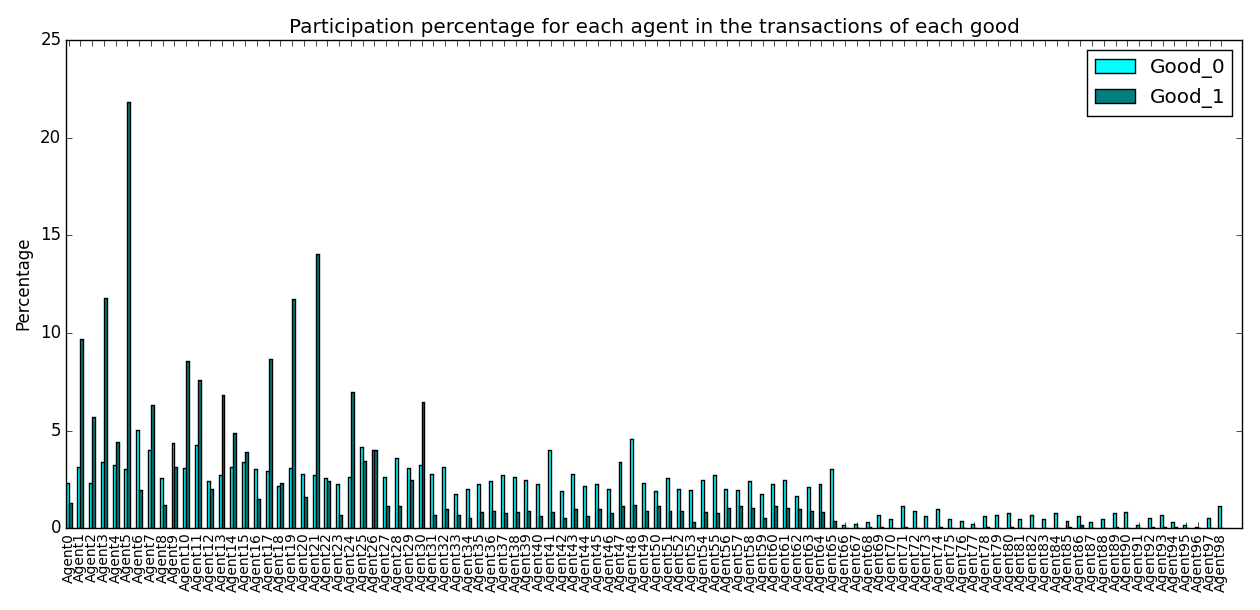
\includegraphics[scale=0.4]{Simulation2_figures/GR_L1B2N1/Figure3_2goods_5k}
\caption{Transaction percentage for GR\_L1B2N1 with 2 sustainable goods after 5000 transactions.}
\end{figure}

\begin{figure}[h!]
\centering
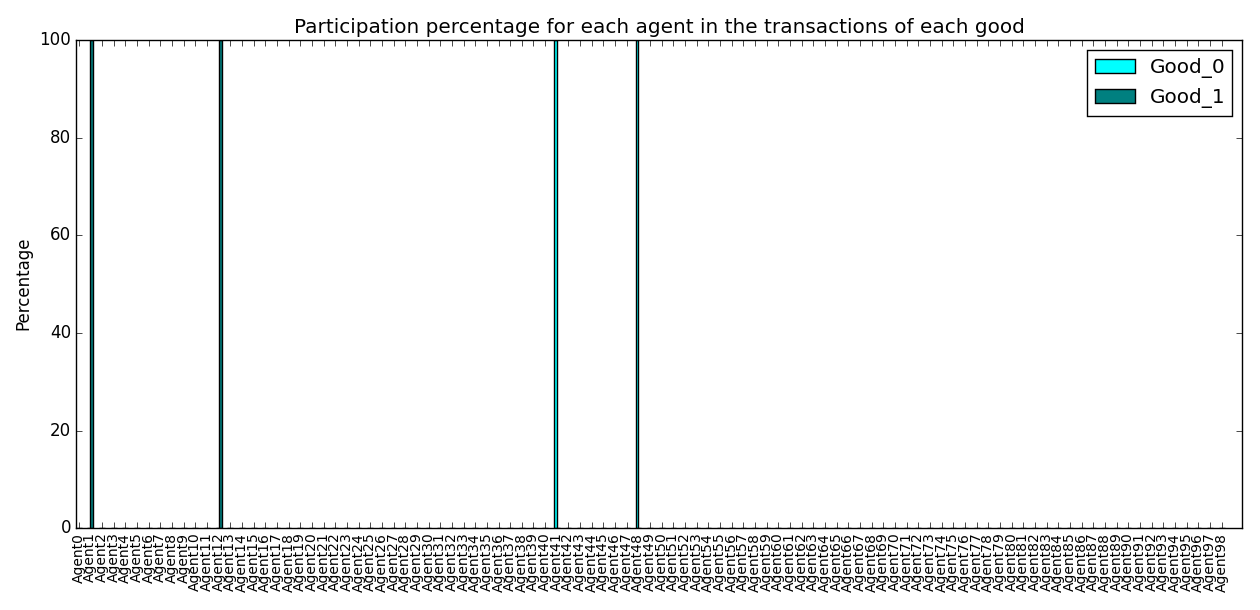
\includegraphics[scale=0.4]{Simulation2_figures/GR_L1B2N1/Figure4_2goods_10k}
\caption{Transaction percentage for GR\_L1B2N1 with 2 sustainable goods after 10000 transactions.}
\end{figure}

For the perishable goods the results are slightly different. With one perishable good and a perish period of 1 all experiments led to a community of the producer and all the agents with a like factor of 0.1 and 0.5. Because the good perishes after it has been given away by the producer the agents who receive the good stay in debt with the producer. The producer therefore prefers the agents with a like factor of 0.1 and 0.5 over 1. \\
\begin{figure}[h!]
\centering
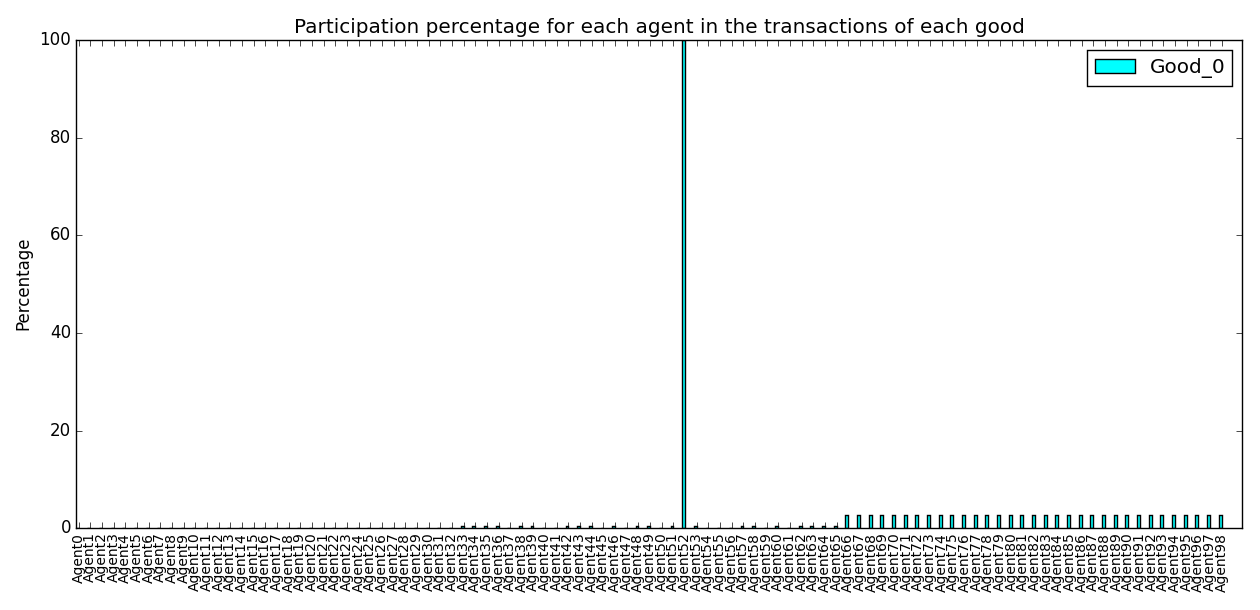
\includegraphics[scale=0.4]{Simulation2_figures/GR_L1B2N1/Figure5_1perishable_4k}
\caption{Transaction percentage for GR\_L1B2N1 with 1 perishable good after 4000 transactions.}
\end{figure}
\\
When the perish period is higher than 1 the goods behave more like a sustainable good. The higher the perish period and the more perishable goods are used the longer it takes before a community arises. In most cases the equilibrium that arises leads to a subgroup of two agents with a like factor of 1 or 0.5 and an agent with a like factor of 0.1. In some cases the subgroup consists of 3 agents as shown in figure 6.13.\\
\begin{figure}[h!]
\centering
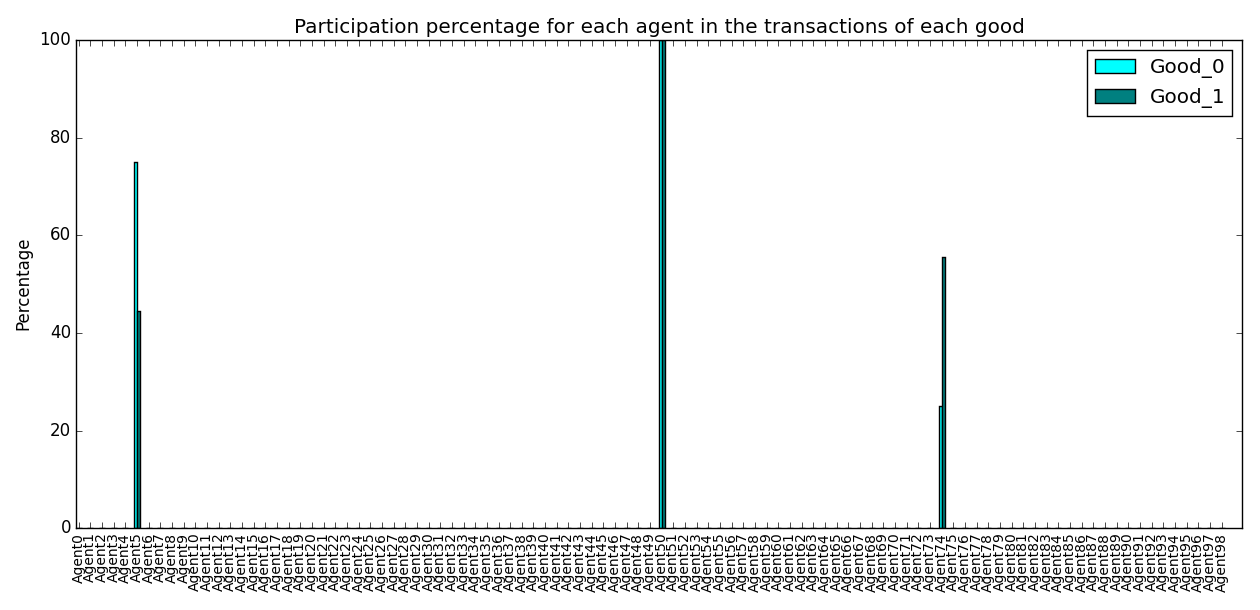
\includegraphics[scale=0.4]{Simulation2_figures/GR_L1B2N1/Figure6_2perishable_5k} 
\caption{Transaction percentage for GR\_L1B2N1 with 2 perishable goods after 5000 transactions.}
\end{figure}

\clearpage
\subsubsection{GR\_L1B2N2}
For the sustainable goods the results show that a community arises more quickly in comparison with GR\_L1B2N1 where the nominal values are the same for every agent. Where it took GR\_L1B2N1 with one good 4000-5000 transactions before a community arose these experiments only took 2000 transactions for one good. The distribution of the transactions in the beginning of the simulation is the same as with GR\_L1B2N1. Using more goods led to the same results, where all goods were only traded between two agents. If N2 would be changed so that the 1 like factor group perceives the nominal values of the goods higher than the 0.1 group then nothing changes to the results.\\
\\
For the perishable goods the results are the same as GR\_L1B2N1, but for this scenario the subgroups also arise more quickly.
\\
\\
When N2 is changed such that the agent with like factor 1 perceives the nominal values of the goods higher than the agent with a like factor 0.1 then the results are as shown in figure 6.14. In this case no equilibrium seems to arise between two agents, but the transactions with agents with like factor 1 are still preferred over transactions with other agents. Thus the transactions only take place within the group of agents with like factors 1. When more goods are used the same behaviour occurs. \\
\begin{figure}[h!]
\centering
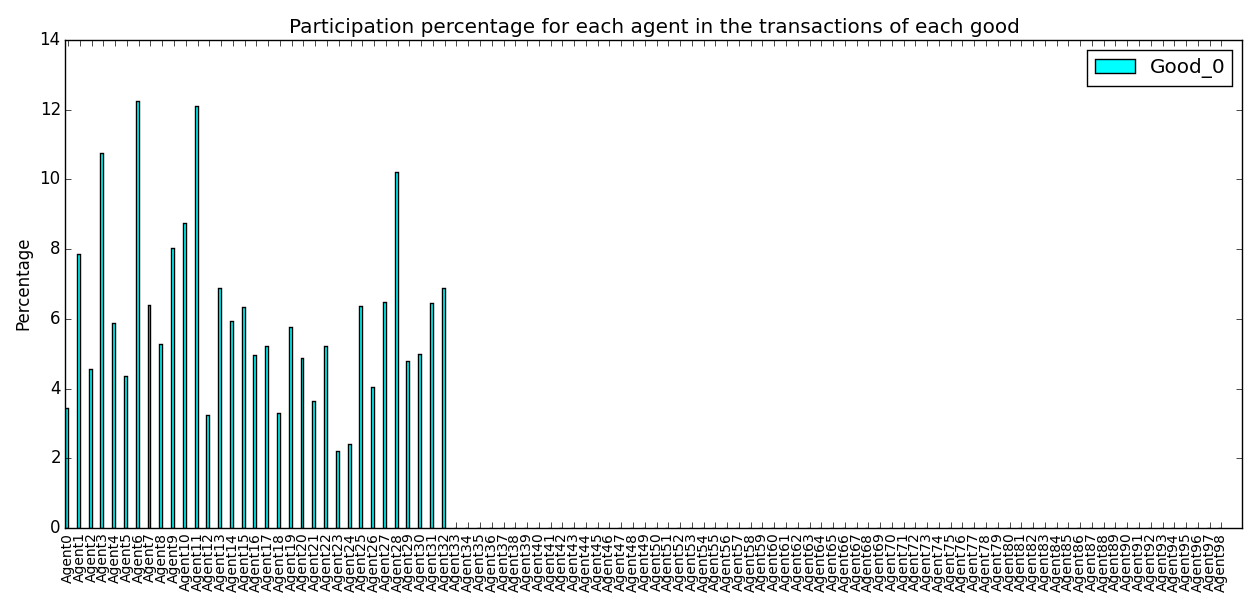
\includegraphics[scale=0.4]{Simulation2_figures/GR_L1B2N2_321/Figure1_10k} 
\caption{Transaction percentage for GR\_L1B2N2 with 1 sustainable good after 10000 transactions.}
\end{figure}

The result shown in figure 6.14 could also be caused by the way the account balances are set in the beginning of the simulation. For the account balance at the start of the simulation natural number were randomly chosen between -9 and 9. This means that in the beginning some agents could have the same account balance, the same like factor an the same nominal value as other agents. This could explain why some agents within the community sometimes have the same yield and thus lead to selecting an agent randomly. We could use real numbers instead of natural numbers between -9 and 9 for the account balance at the start of the simulation to make sure that every account balance would be different. But this led to the same results. Even after 300000 transactions some agents were still randomly selected.

\clearpage
\subsubsection{GR\_L2B2N1}
With this scenario only 5 agents have a like factor of 0.1 and the other agents have either 1 or 0.5. The major difference between this scenario and GR\_L1B2N1 is that the agents with a like factor of 0.1 are ignored more. The reason for this is simply, because the group with a like factor of 0.1 is smaller.
\subsubsection{GR\_L2B2N2}
The results are the same as GR\_L1B2N2. Changing the amount of agents with a like factor of 0.1 did not change anything.
\\
\\
\subsection{Recap}
The scenarios BS\_S and BS\_P confirm a correct implementation of the goodwill rule and a correct calculation of the yield and account balance. The results of the other scenarios show however that what was expected did not happen. Instead of subgroups consisting of agents with a like factor of 0.1 the subgroups consist of agents with like factor 1 or 0.5 with sometimes agent with like factor 0.1. Instead of giving to agents who are liked more the agents in these scenarios prefer to give to agents who are not liked at all. On one hand this seems logical if you think about loans and in this case hostile loans where each time a good is given it leads to a high debt. With the yield curve used for this model receiving a good from someone who is not liked leads to a higher debt than receiving from someone who is liked, because the slope is heigher with a like factor of 1. On the other hand this seems illogical for a giving environment, where people rather give/pay of their debt with someone they like than with someone they don't like. This has led to a reconsideration of the yield curve used in this thesis.








\section{Reconsideration of the yield curve}
The results from the goodwill rule have revealed a problem. The problem is as follows: We have an agent P who is in possession of a good and two other agents Q and R who P can give his good to. P has an account balance of 0 with both agents, P has a like factor of 0.1 with Q and a like factor of 1 with R. This would lead to the yield curve shown in figure 6.15. \\
\begin{figure}[h!]
\centering
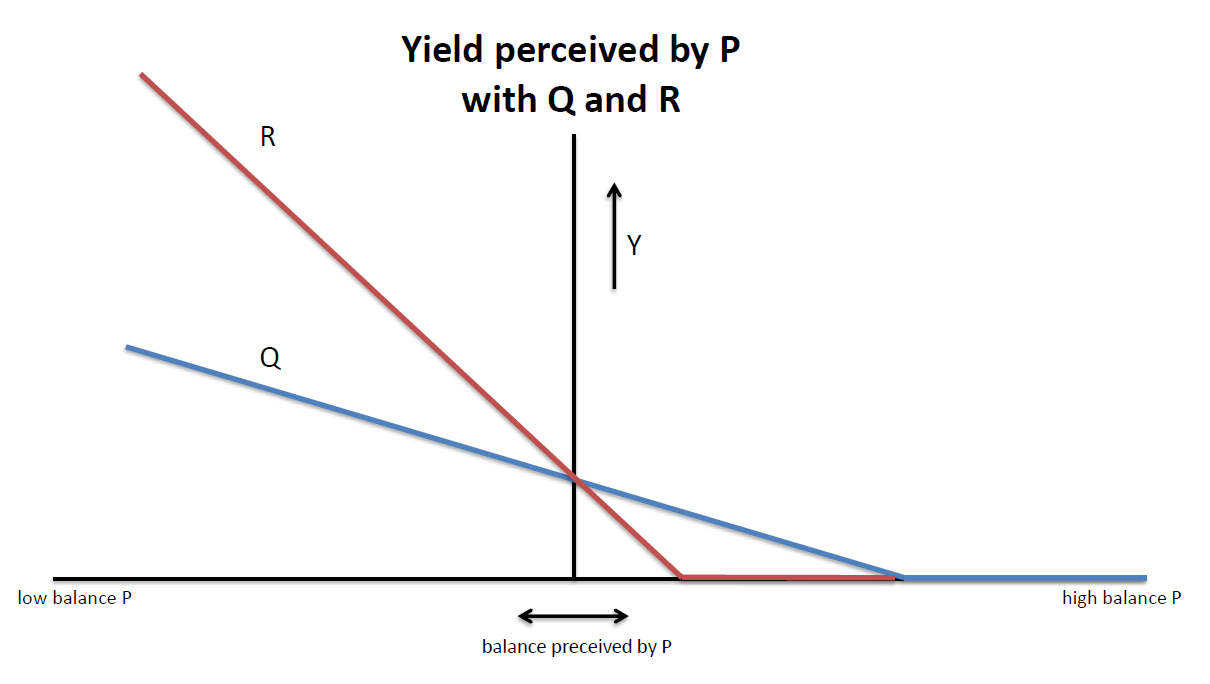
\includegraphics[scale=0.4]{YieldCurves/yieldcurve_P_QR}
\caption{Yield curve, yield perceived by P with Q and R.}
\end{figure}
\\
P now has to decide to whom he will give the good. It would be logically to assume that because P likes Q more he will give to Q. The yield curve is currently defined as that the yield determines the choice to who the good will be given to. When the yield is the same for multiple agents an agent will be randomly selected. According to the yield it does not matter who is chosen, because all transactions are valued the same. So P will randomly choose between Q and R. Due to the results from the goodwill rule where the transactions are in favour of the lesser liked agents it has become clear that the way an agent is chosen when the yield is the same is not completely representative for a giving environment.

A solution to this problem would be to base the perception of the nominal value of a good on the like factors between all agent pairs. This would mean that for every good a NxN matrix needs to be created where the perception of the nominal value is different for every agent pair. However this solution requires a lot of additional input data which would need to be created and stored by the user. A better solution would be to rewrite the calculation of the yield so that we get a yield curve shown in figure 6.16 even when only one good is used. \\
\begin{figure}[h!]
\centering
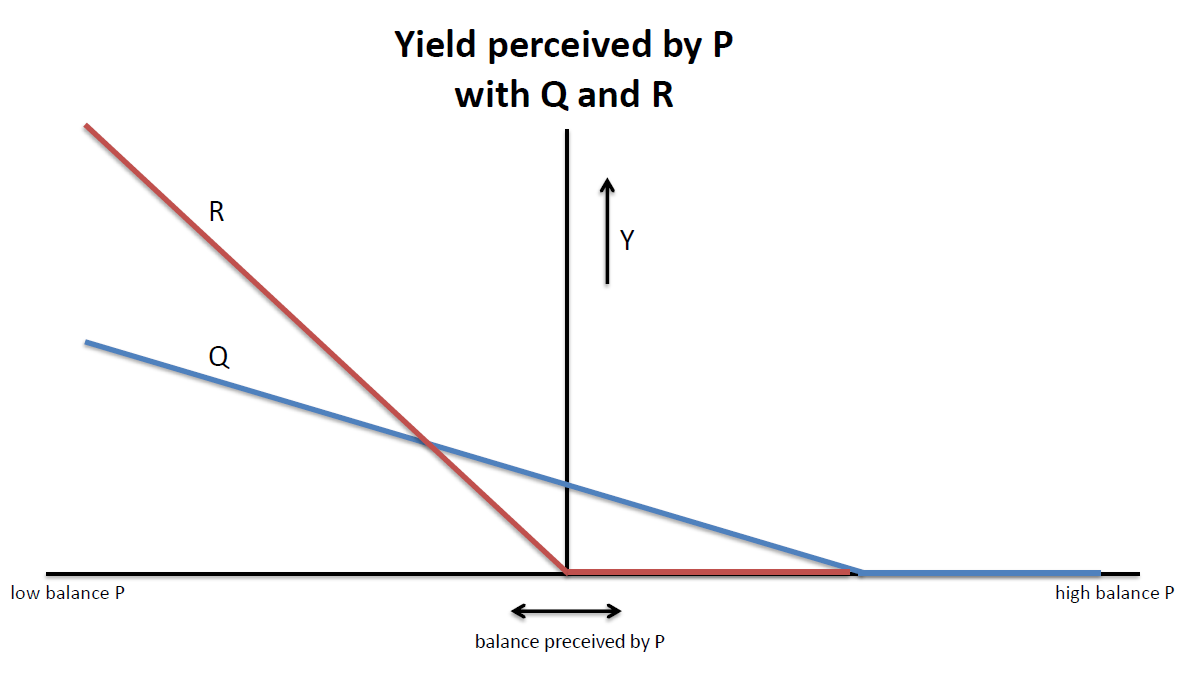
\includegraphics[scale=0.4]{YieldCurves/yieldcurve_P_QR2}
\caption{Yield curve, yield perceived by P with Q and R.}
\end{figure}

The yield curve in figure 6.16 shows that with an account balance of 0 and a like factor of 1 the value of the transaction is lower than when the like factor would be 0.1. In this case P would choose Q over R, because a transaction with a 'friend' is worth more than with a stranger. This means that when the nominal value is defined as a constant than the intercept(\textit{b}) in \textit{$Y = aX + b$} should be a lower value when the like factor is higher. To accomplish this we can assume that \textit{b} will scale equally with the like factor, thus \textit{$Y' = aX + b(1 - a)$}. The calculation of the yield needs to be rewritten as follows:
\begin{equation}
\begin{split}
Y & = -aX + b \\
Y' & = -aX + b(1 - a) \\
& = -aX + b - ab \\
& = -a(X + b) + b 
\end{split}
\end{equation}
This new calculation of the yield leads to yield curves just like the one in figure 6.16 and solves the problem of choosing an agent when the balance is 0. To see what the effect is of these changes on the results of the goodwill scenarios additional experiments have been performed with the revised yield curve. The results of the experiments that show major differences in results are explained below.

\begin{description}
\item[GR\_L1B1N1] When the good starts at an agent with like factor 1 the good is given away to an agent with like factor 0.1. Once the good is in possession of an agent with like factor 0.1 a subgroup arises between two agents with a like factor 0.1. When the good starts at an agent with like factor 0.5 the good is also given to an agent with like factor 0.1. This time a subgroup arises between the agent with like factor 0.5 and the agent with like factor 0.1 who received the good the first time. These results are the same for every additional good.

For the perishable goods the results are very different. With one perishable good and a perish period of 1 all experiments led to a community of the producer and all the agents with a like factor of 0.1 and 0.5 as shown in figure 6.17 Because the good perishes after it has been given away by the producer the agents who receive the good stay in debt with the producer. The producer therefore prefers the agents with a like factor of 0.1 and 0.5 over 1. \\
\begin{figure}[h!]
\centering
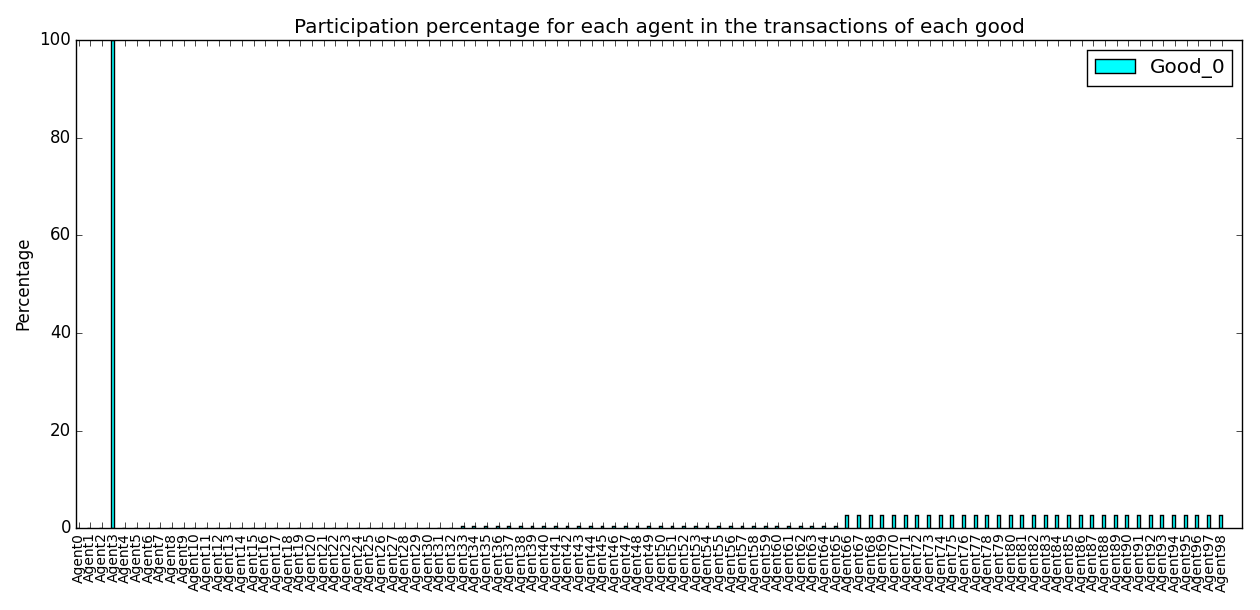
\includegraphics[scale=0.4]{Simulation_figures/GR_L1B1N1/1perishable_1-1_15k}
\caption{Transaction percentage for GR\_L1B1N1 with 1 perishable good.}
\end{figure}

When an odd number is used for the perish period the results are similar to the results shown in figure 6.17 but instead the producer only gives to agents with like factors 0.1. When an even number is used for the perish period the goods are immediately traded between two agents with a like factor of 0.1. If we would use a combination of perishable goods with odd perish periods and even perish periods the results would be a combination of the previous results. The perishable goods sometimes take place within a subgroup for a short period of time. When some agents reach the highest possible equilibrium with each other the transactions eventually led to subgroups as shown in figure 6.18 With other experiments this equilibrium was not reached and instead the subgroup consisted of the producers and the agents with like factors 0.1 as shown in figure 6.19 \\
\begin{figure}[h!]
\centering
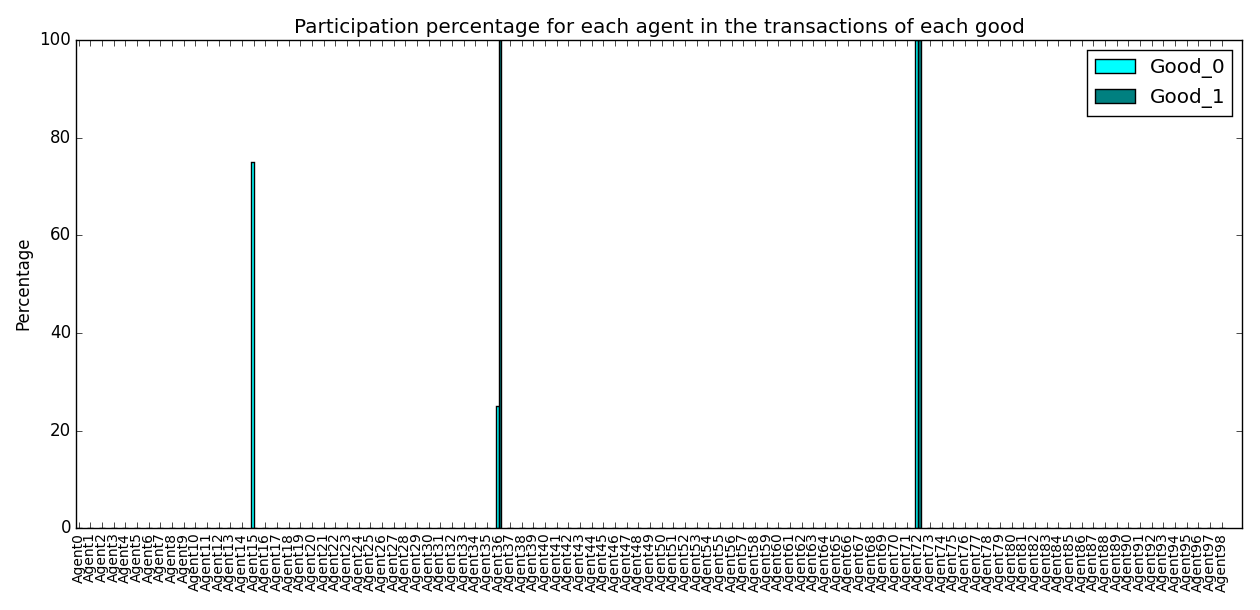
\includegraphics[scale=0.4]{Simulation_figures/GR_L1B1N1/2perishable_2233_100k}
\caption{Transaction percentage for GR\_L1B1N1 with 2 perishable goods.}
\end{figure}
\begin{figure}[h!]
\centering
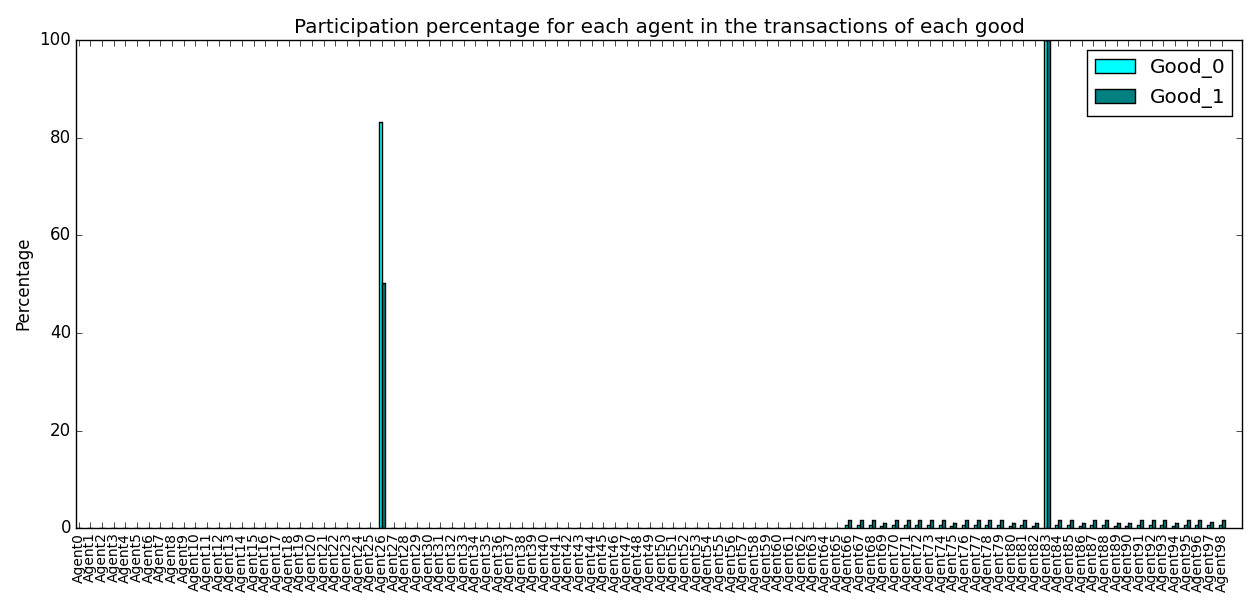
\includegraphics[scale=0.4]{Simulation_figures/GR_L1B1N1/2perishable_largercommunity}
\caption{Transaction percentage for GR\_L1B1N1 with 2 perishable goods.}
\end{figure}

\clearpage
\item[GR\_L1B1N2] When N2 is used where the nominal values are perceived higher by the agent with like factor 0.1 than the agents with like factor 1 then the results are similar to the results from GR\_L1B1N1. The only difference is that the subgroups only consist of agent with a like factor of 0.1, because these agents perceive the nominal value of the good the highest. For every additional good used the results are the same.
\\
\\
When N2 is changed so the agent with like factor 1 perceive the nominal values of the goods higher than the agent with a like factor 0.1 then the results are as shown in figure 6.20 The transactions within this subgroup do not stabilize, because the transactions are still random within this subgroup. This randomness occurs, because within these communities the yield sometimes reaches the same value for multiple agents. For example when an agent has to choose between two agents who have the same like factor and balance the choice will still be random.
When the good starts at an agent with a like factor of 0.1 a subgroup immediately arises where the good is traded between two agents with a like factor of 0.1.\\
\begin{figure}[h!]
\centering
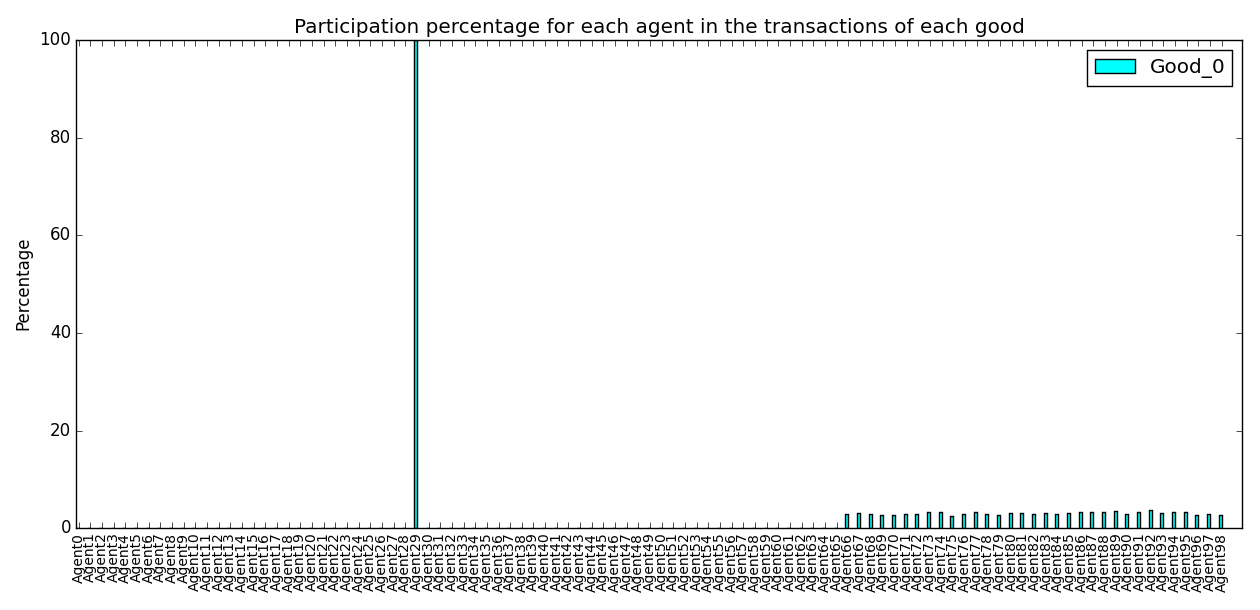
\includegraphics[scale=0.4]{Simulation_figures/GR_L1B1N2/321_1good} 
\caption{Transaction percentage for GR\_L1B1N2 with 1 good.}
\end{figure}


When more goods are used and some goods start at agents with like factors 1 or 0.5 and other goods start at agents with like factors 0.1 then a subgroup shown in figure 6.21 arises where the transactions are not equally distributed over the agents. The transactions within this subgroup do not stabilize, because the distribution of the transactions changes as more transactions take place. The yield never reaches an equilibrium. \\
\begin{figure}[h!]
\centering
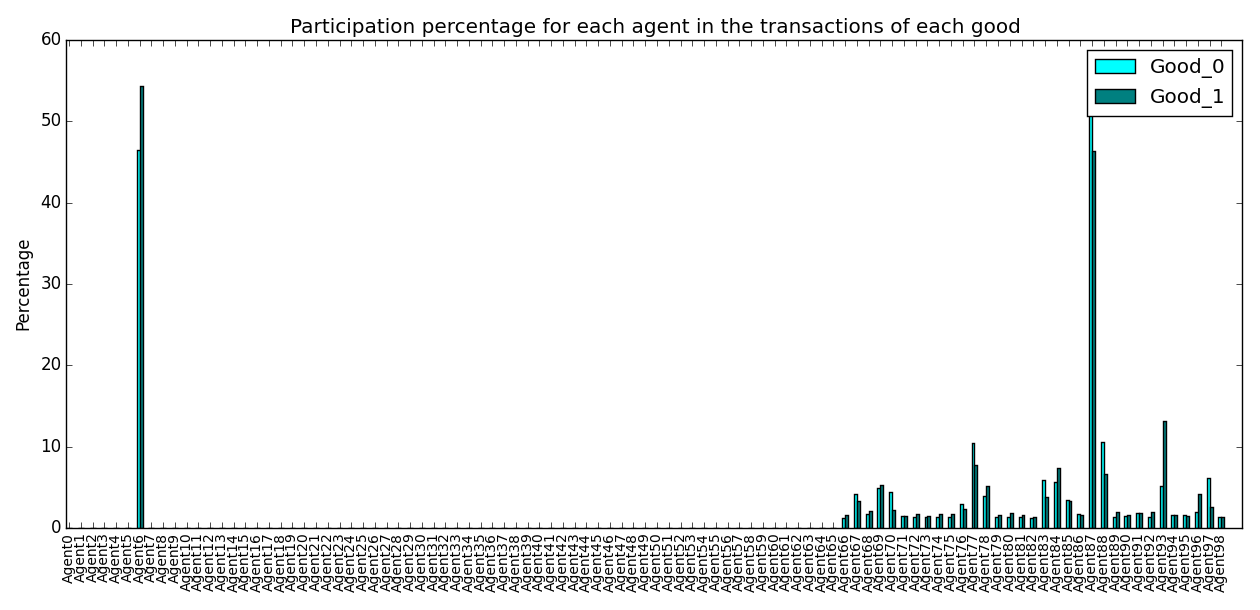
\includegraphics[scale=0.4]{Simulation_figures/GR_L1B1N2/2goods_spikes}
\caption{Transaction percentage for GR\_L1B1N2 with 2 goods.}
\end{figure}

When perishable goods are used the results are equal to the results from GR\_L1B1N1.
\clearpage
\item[GR\_L1B2N1] For the first 1000-2000 transactions the transactions are in favour of the agents with a higher like factor as shown in figure 6.22. The debts are in the beginning higher, thus the yield for agents with a like factor of 1 is higher than for agents with like factor 0.1. Once these debts are payed the transactions start to lean more towards the agents with like factor 0.1 as shown in figure 6.23. Eventually after approximately 6000 transactions a subgroup arises consisting of two agents with like factors 0.5 or 0.1.
\begin{figure}[h!]
\centering
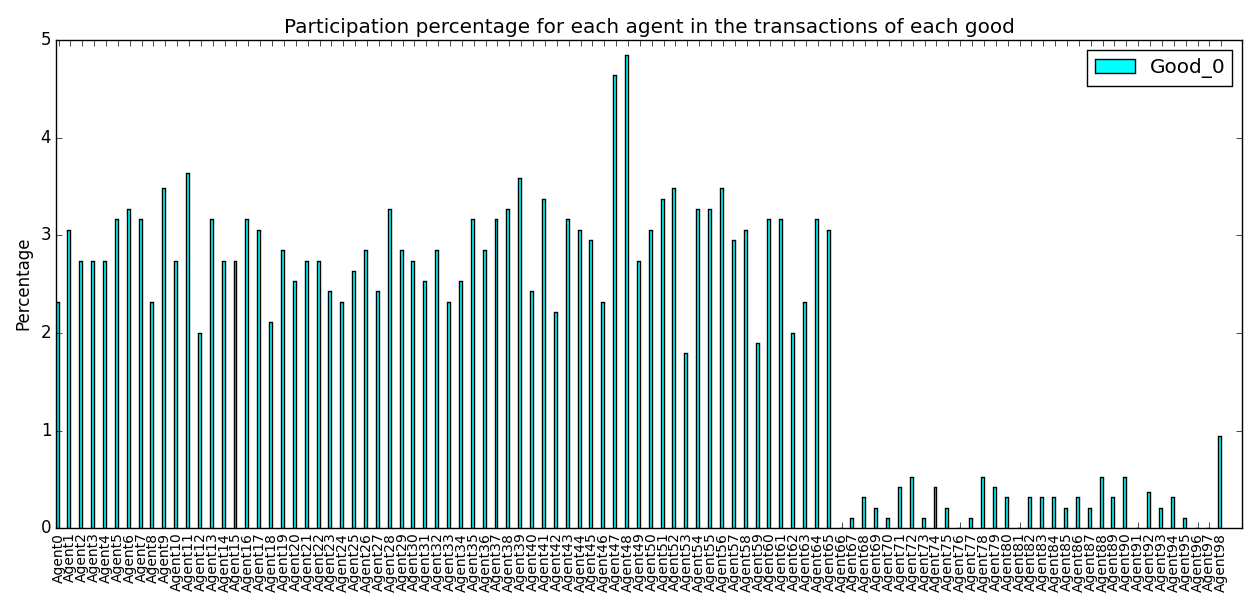
\includegraphics[scale=0.4]{Simulation2_figures/GR_L1B2N1_1good_2k} 
\caption{Transaction percentage for GR\_L1B2N1 with 1 good.}
\end{figure}

\begin{figure}[h!]
\centering
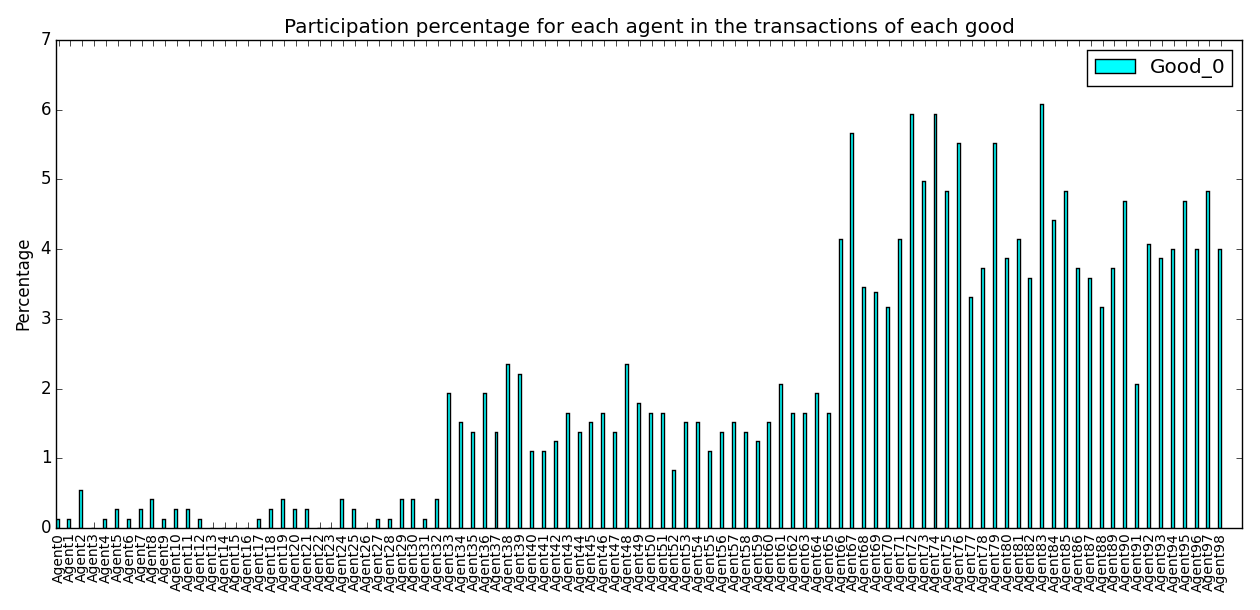
\includegraphics[scale=0.4]{Simulation2_figures/GR_L1B2N1_1good_5k} 
\caption{Transaction percentage for GR\_L1B2N1 with 1 good.}
\end{figure}


When perishable goods are used the result is eventually the same as with GR\_L1B1N1 where the higher the perish period the more the goods behave like sustainable goods. The only difference is the distribution of the transactions in the beginning of the simulation. With this scenario the goods are traded more between agents with different like factor before a community arises, because the account balance is not 0 in the beginning. 

\item[GR\_L1B2N2] When N2 is used where the nominal values are perceived higher by the agent with a 0.1 like factor than the agents with a 1 like factor then the results are the same as the results from GR\_L1B2N1. The only difference is that with different nominal values the subgroups arise more quickly. Where it took GR\_L1B2N1 approximately 6000 transactions it took this scenario only approximately 3000-4000 transactions. When more goods are used the results are not affected.

When N2 is changed so the agent with a 1 like factor perceive the nominal values of the goods higher than the agent with a 0.1 like factor then a subgroup arises with the agent who started with the goods and the agents with like factors 0.1. The distribution of the transactions in the beginning of the simulation are the same as show in figure 6.22 and 6.23, but eventually a community arises as shown in figure 6.24. The transactions within this community are not executed in a repeating sequence, because for some transactions the yield can be the same for multiple agents, thus an agent needs to be randomly selected. Some experiments led to an equilibrium between two agents which led to a subgroup consisting of only two agents with like factors 0.1.
\begin{figure}[h!]
\centering
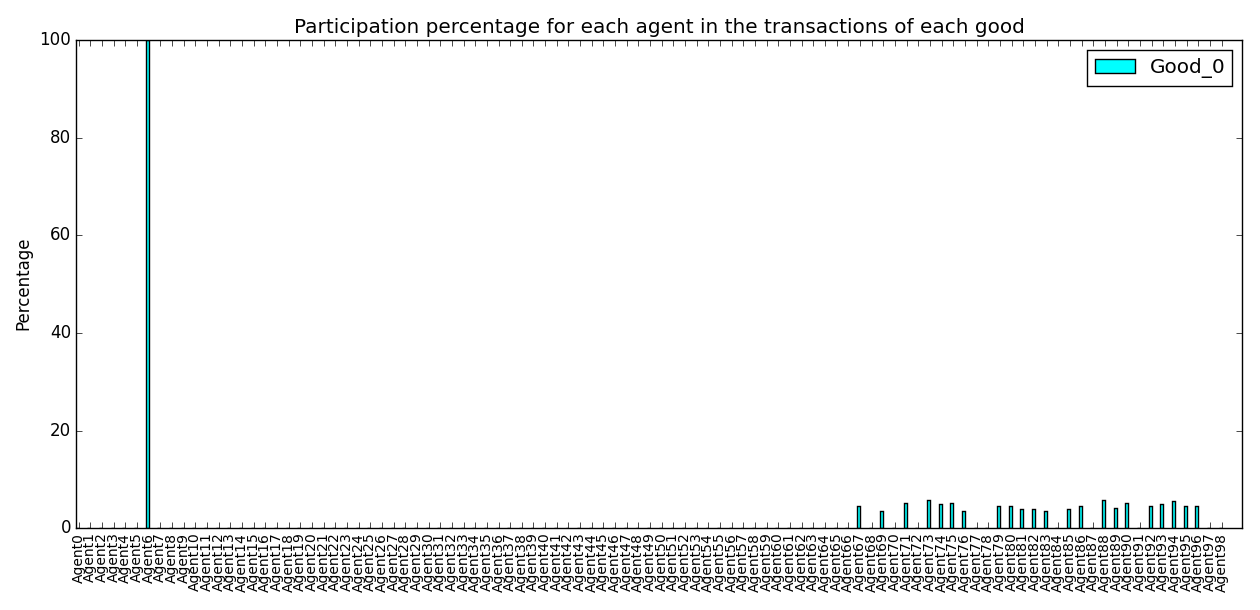
\includegraphics[scale=0.4]{Simulation2_figures/GR_L1B2N2_321_4k} 
\caption{Transaction percentage for GR\_L1B2N2 with 1 good.}
\end{figure}

If we use real numbers instead of natural numbers between -9 and 9 for the account balance at the start of the simulation just like with the first GR\_L1B2N2 experiments the same results as in figure 6.24 occur. The agents within the community are still randomly selected.

\end{description}

The major difference between the revised yield curve and the original one is that when B1 is used a community does not immediately arise. The transactions are also more distributed in favour of the agents with a like factor of 0.1 as shown in figure 6.23. 










\chapter{Conclusions and Discussions}
The created simulation program provides a wide range of possible scenarios to simulate the giving game designed for this thesis. The scenarios of the random rule and balance rule were very basic scenarios to test the implemented giving game. The behaviour of both the random rule and the balance rule was very predictable and showed a correct implementation of the giving game. The balance rule also confirmed a correct calculation of the community effect to see where the subgroups emerged and how many agents were part of these subgroups.

The first experiments of the goodwill rule showed surprising results. These results have led to a reconsideration of the yield curve which caused an improvement in the simulation model for the giving game. The results from the goodwill experiments confirmed the hypothesis and clearly show that in most cases agents rather give to 'friends' than to stranger. The results have led to the answer for the first research question. \\ 
\\
\textit{In a Giving Game simulation will transactions eventually take place within a limited subgroup of the entire population?} \\
The answer to this question is simply, yes. All the goodwill rule experiments eventually led to subgroups. As expected in the first place the experiments with the revised yield curve led to subgroups consisting mostly of agents who like each other. Most experiments led to subgroups consisting of two agents. Larger subgroups are an exception.
\\
\\
The results also show that the emergence of subgroups are mostly affected by the different nominal values and account balances. A higher perception of the nominal value of a good and a low balance means a higher possible yield. Some experiments therefore showed a distribution of the transactions in favour of the less liked agents or a community where also an agent who is less liked was part of. The emergence of larger subgroups as the effect of different nominal values and different account balances has led to the answer for the second research question.
\\
\\
\textit{In a Giving Game simulation will we see a repeating sequence of transactions or will the transaction sequence look random?} \\
The balance rule showed a partial stabilization of the transactions when perishable goods were used with a perish period of 1. Experiments with the goodwill rule did not lead to a repeating sequence of transactions. Even when communities larger than two agents arose some transactions within these communities were still random, therefore no repeating sequence of transactions took place.

\section{Further research}
The scenarios used for the simulation have some restrictions. For the like factors the assumption was made that the like factors are constant over the whole population. In 'real life' these like factors could be different for everyone or even change over time. The nominal values were restricted to the same groups, but could also vary alot more for further research. The account balance at the beginning of the simulation could also be randomly generated with real numbers instead of natural numbers. Even though the scenario GR\_L1B2N2 of both yield curves did not show any different results, further research could prove otherwise.

The experiments of the goodwill rule have showed a basic representation real life environment where people invest and all agents try to maximize profit by giving more to agents who are liked than to agents who are not liked. The giving game used for the experiments and the related results do not cover everything of an economy of giving. Further research could use more varying input for the simulations or even add parameters to make the simulation more realistic so human behaviour can be simulated more precise. A possible variant on the giving game used in this thesis could for example be that agents are able to hold on to a good. This is leads to a similar simulation as used for the 'Kiyotaki-Wright Model'\cite{moranmoney}. Holding on to a good is a more realistic approach, but comes with a few extra parameters. Realistically holding on to a good means that the good needs to be stored somewhere. In the real world this would mean that storage costs have to be paid and certain goods, perishable goods for example, would not be able to be stored forever. Holding on to a good could be a strategic choice by the agent.
\\
\\
The already revised yield curve can also be further tested or improved. This thesis has used a simplified version of a yield curve. Different calculations of the yield could lead to non-linear yield curves. \\
\\
Lastly, to the created simulation of the giving game used more selection rules can be added that use more complex algorithms to select an agent. This can lead to a more real environment. Further information about extending the created simulation can be found in appendix A.

\bibliography{references}
\bibliographystyle{plain}


\appendix
\chapter{Simulator manual}
In this appendix all information about running the simulator will be discussed.

\section{Dependencies}
In order to run the simulator several dependencies have to be installed on the system. The following has to be installed:
\begin{itemize}
\item Python3.3+
\item Numpy
\item python-matplotlib
\item python-openpyxl
\item VisPy
\item PyQt4
\end{itemize}

\section{Running the simulator}
The simulator can be started by using the \textit{python giving\_game\_simulator.py} command from the \textit{Simulator} folder.

\section{Usage}
The input interface is as shown in figure A.1.
\begin{enumerate}
\item Choose the number of agents for the simulation
\item Choose the number of goods for the simulation
\item Choose between perishable goods or sustainable goods. Default values are 0, meaning the good is a sustainable good.
\item Add/remove a xls or xlsx file for the like factors. Default like factors are -0.5.
\item Add/remove a xls or xlsx file for the starting account balances. Default account balance is 0 for every agent.
\item Add/remove a xls or xlsx file for the nominal values. Default nominal value is 1.
\item Choose a selection rule. Default is the random rule.
\item Choose between executing the transaction parallel or one by one.
\item Start the simulation. Gives an error when parameters are missing or wrong parameters are given.
\end{enumerate}

The output interface is as shown in figure A.2.
\begin{enumerate}
\item Choose an agent. A window opens shows how much the chosen agent has given and received.
\item Choose 2 agents. The yield curve is shown for between both agents.
\item Choose the subgroup size with the slider. Choose a good to calculate what percentage of the total transaction of the selected good are within a subgroup of the set size. The 'reset percentage' button allows the user to reset the number of transactions that has been executed and the number of times each agent has contributed to a transaction. This allows the user to see if from a certain point in the simulation the transactions only take place within a subgroup of the set size.
\item Shows all the previous executed transactions.
\item Total executed transactions are shown. The user can pause and start the simulation or set a delay between each transaction with the slider.
\item Choose to show the visualization of the transactions or show the transaction percentage of each good for each agent.
\item The window where the visualization of the transactions or the \textit{community percentage} will be shown.
\end{enumerate}


\begin{figure}[h]
\centering
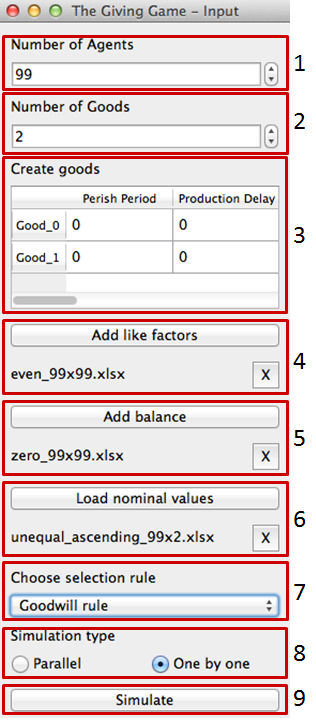
\includegraphics[scale=0.5]{Manual/Input}
\caption{Input interface for the simulation program.}
\end{figure}
\begin{figure}[h]
\centering
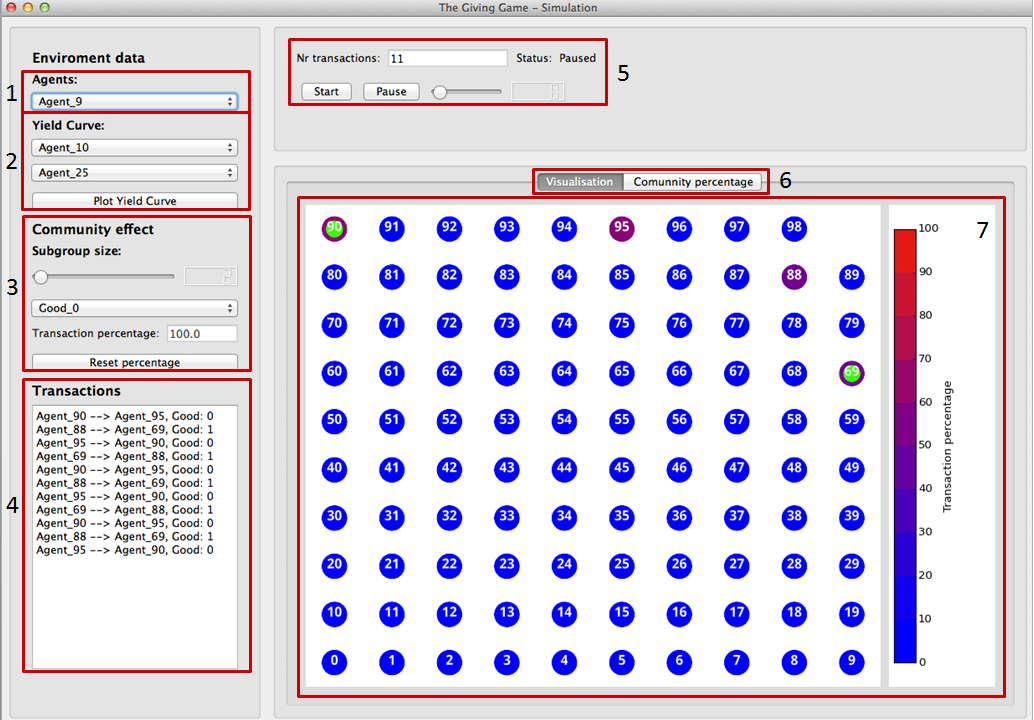
\includegraphics[scale=0.5]{Manual/Output}
\caption{Output interface for the simulation program.}
\end{figure}

\section{Extending the simulation program}
Selection rules can be added by added a python functions for the selection rule to \textit{Selection\_rules.py} in the folder \textit{Simulator}. To allow the user to choose the added selection rule the interface of \textit{GUI\_Input.py} needs to be changed and the selection rule needs to be added to \textit{Environment.py}.

To further extend calculations, updating variables or the simulation model the files \textit{Simulate.py} and \textit{Environment.py} should be changed.

\end{document}
